% Pengaturan ukuran teks dan bentuk halaman dua sisi
\documentclass[12pt]{book}

% Pengaturan ukuran halaman dan margin
\usepackage[a4paper,top=30mm,left=30mm,right=20mm,bottom=25mm]{geometry}

% Pengaturan ukuran spasi
\usepackage[singlespacing]{setspace}

% Pengaturan caption untuk tabel
\usepackage{caption}

% Judul dokumen
\title{Proposal Tugas Akhir ITS}
\author{Musk, Elon Reeve}

% Pengaturan detail pada file PDF
\usepackage[pdfauthor={\@author},bookmarksnumbered,pdfborder={0 0 0}]{hyperref}


% Pengaturan ukuran indentasi
\setlength{\parindent}{2em}

% Package lainnya
\usepackage{changepage}
\usepackage{etoolbox} % Mengubah fungsi default

% Pengaturan jenis karakter
\usepackage[utf8]{inputenc}

\usepackage[style=ieee, backend=biber]{biblatex}
\usepackage{enumitem} % Pembuatan list
\usepackage{lipsum} % Pembuatan template kalimat
\usepackage{graphicx} % Input gambar
\usepackage{longtable} % Pembuatan tabel
\usepackage[table,xcdraw]{xcolor} % Pewarnaan tabel
\usepackage{eso-pic} % Untuk menggunakan background image di halaman
\usepackage{txfonts} % Font times
\usepackage{changepage} % Pembuatan teks kolom
\usepackage{multicol} % Pembuatan kolom ganda
\usepackage{multirow} % Pembuatan baris ganda
\usepackage{tabularx} % Untuk mengatur kolom, seperti grid pada CSS
\usepackage{wrapfig}
\usepackage{float}

% Pengaturan format daftar isi, daftar gambar, dan daftar tabel
\usepackage[titles]{tocloft}
\setlength{\cftsecindent}{2em}
\setlength{\cftsubsecindent}{2em}
\setlength{\cftbeforechapskip}{1.5ex}
\setlength{\cftbeforesecskip}{1.5ex}
\setlength{\cftbeforetoctitleskip}{0cm}
\setlength{\cftbeforeloftitleskip}{0cm}
\setlength{\cftbeforelottitleskip}{0cm}
\renewcommand{\cfttoctitlefont}{\hfill\Large\bfseries} % command untuk membuat heading bold dan besar
\renewcommand{\cftaftertoctitle}{\hfill}
\renewcommand{\cftloftitlefont}{\hfill\Large\bfseries}
\renewcommand{\cftafterloftitle}{\hfill}
\renewcommand{\cftlottitlefont}{\hfill\Large\bfseries}
\renewcommand{\cftafterlottitle}{\hfill}

% Definisi untuk "Hati ini sengaja dikosongkan"
\patchcmd{\cleardoublepage}{\hbox{}}{
  \thispagestyle{empty}
  \vspace*{\fill}
  \begin{center}\textit{[Halaman ini sengaja dikosongkan]}\end{center}
  \vfill}{}{}

  % Pengaturan penomoran halaman
\usepackage{fancyhdr}
\fancyhf{}
\renewcommand{\headrulewidth}{0pt}
\pagestyle{fancy}
\fancyfoot[C,CO]{\thepage}
\patchcmd{\chapter}{plain}{fancy}{}{}
\patchcmd{\chapter}{empty}{plain}{}{}

% Pengaturan format judul bab
\usepackage{titlesec}
\renewcommand{\thesection}{\thechapter.\arabic{section}}
\titleformat{\chapter}[hang]{\centering\bfseries\large}{BAB\ \arabic{chapter}\ }{0ex}{\vspace{0ex}\centering}
\titleformat*{\section}{\large\bfseries}
\titleformat*{\subsection}{\normalsize\bfseries}
\titlespacing{\chapter}{0ex}{0ex}{4ex}
\titlespacing{\section}{0ex}{1ex}{0ex}
\titlespacing{\subsection}{0ex}{0.5ex}{0ex}
\titlespacing{\subsubsection}{0ex}{0.5ex}{0ex}
\setcounter{secnumdepth}{3} % Untuk memberi penomoran pada \subsubsection

\counterwithin{figure}{chapter}
\counterwithin{table}{chapter}

% Mengganti figure dan table menjadi gambar dan tabel
\renewcommand{\figurename}{Gambar}
\renewcommand{\tablename}{Tabel}

% Tambahkan format tanda hubung yang benar di sini
\hyphenation{
  ro-ket
  me-ngem-bang-kan
  per-hi-tu-ngan
}

% Menambahkan resource daftar pustaka
\addbibresource{pustaka/pustaka.bib}

% Isi keseluruhan dokumen
\begin{document}
  % Nomor halaman pembuka dimulai dari sini
  \pagenumbering{roman}

  % Atur ulang penomoran halaman
  \setcounter{page}{1}

  % Sampul Bahasa Indonesia
  \newcommand\covercontents{sampul/konten-id.tex}
  \AddToShipoutPictureBG*{
  \AtPageLowerLeft{
    % Ubah nilai berikut jika posisi horizontal background tidak sesuai
    \hspace{-3.25mm}

    % Ubah nilai berikut jika posisi vertikal background tidak sesuai
    \raisebox{0mm}{
      
\includegraphics[width=\paperwidth,height=\paperheight]{sampul/gambar/sampul-luar-tipis.png}
    }
  }
}

% Menyembunyikan nomor halaman
\thispagestyle{empty}

% Pengaturan margin untuk menyesuaikan konten sampul
\newgeometry{
  top=65mm,
  left=30mm,
  right=30mm,
  bottom=20mm
}

\begin{flushleft}

  % Pemilihan font sans serif
  \sffamily

  % Pemilihan font bold
  \fontseries{bx}
  \selectfont
  \begin{spacing}{1.5}
    \input{\covercontents}
  \end{spacing}

\end{flushleft}

\restoregeometry

  \cleardoublepage
  
  % Sampul Bahasa Inggris
  \renewcommand\covercontents{sampul/konten-en.tex}
  \AddToShipoutPictureBG*{
  \AtPageLowerLeft{
    % Ubah nilai berikut jika posisi horizontal background tidak sesuai
    \hspace{-3.25mm}

    % Ubah nilai berikut jika posisi vertikal background tidak sesuai
    \raisebox{0mm}{
      
\includegraphics[width=\paperwidth,height=\paperheight]{sampul/gambar/sampul-luar-tipis.png}
    }
  }
}

% Menyembunyikan nomor halaman
\thispagestyle{empty}

% Pengaturan margin untuk menyesuaikan konten sampul
\newgeometry{
  top=65mm,
  left=30mm,
  right=30mm,
  bottom=20mm
}

\begin{flushleft}

  % Pemilihan font sans serif
  \sffamily

  % Pemilihan font bold
  \fontseries{bx}
  \selectfont
  \begin{spacing}{1.5}
    \input{\covercontents}
  \end{spacing}

\end{flushleft}

\restoregeometry


  % Lembar pengesahan
  \chapter*{LEMBAR PENGESAHAN}

% Menyembunyikan nomor halaman
\thispagestyle{empty}

\begin{center}
  % Ubah kalimat berikut dengan judul tugas akhir
  \textbf{ALAT PENGISI TOKEN LISTRIK MENGGUNAKAN SISTEM \emph{2-AXIS GANTRY} BERBASIS IOT}
\end{center}

\begingroup
% Pemilihan font ukuran small
\small

\begin{center}
  % Ubah kalimat berikut dengan pernyataan untuk lembar pengesahan
  \textbf{PROPOSAL TUGAS AKHIR} \\
  Diajukan untuk memenuhi salah satu syarat memperoleh gelar
  Sarjana Teknik pada
  Program Studi S-1 Teknik Komputer \\
  Departemen Teknik Komputer \\
  Fakultas Teknik Elektro dan Informatika Cerdas \\
  Institut Teknologi Sepuluh Nopember
\end{center}

\begin{center}
  % Ubah kalimat berikut dengan nama dan NRP mahasiswa
  Oleh: \textbf{Rayhan Narindran Cendikia} \\
  NRP. 5024211022
\end{center}

\begin{center}
  Disetujui Oleh:
\end{center}

\vspace{10ex}

\begingroup
% Menghilangkan padding
\setlength{\tabcolsep}{0pt}

\noindent
\begin{tabularx}{\textwidth}{X c}
  % Ubah kalimat-kalimat berikut dengan nama dan NIP dosen pembimbing pertama
  Arta Kusuma Hernanda, S.T., M.T.      &                 \\
  NPP: 1996202311024                    & (Pembimbing)    \\
                                        &                 \\
                                        &                 \\
                                        &                 \\
  % Ubah kalimat-kalimat berikut dengan nama dan NIP dosen pembimbing kedua
  PEMBIMBING 2                          &                 \\
  NIP: NIP PEMBIMBING 2                 & (Ko-Pembimbing) \\
\end{tabularx}
\endgroup

\vspace{\fill}

\begin{center}
  Mengetahui,\\
  % Ubah kalimat berikut dengan nama departemen
  Kepala Departemen Teknik Komputer ITS\\
  \vspace{10ex}
  % Ubah kalimat berikut dengan jabatan kepala departemen
  \underline{Dr. Supeno Mardi Susiki Nugroho, S.T., M.T.}\\
  NIP 19700313199512 1 001\\
  \vspace{10ex}
  % Ubah text dibawah menjadi tempat dan tanggal
  \textbf{SURABAYA} \\
  \textbf{Mei, 2077}
\end{center}
\endgroup

  \cleardoublepage

  % Abstrak
  \chapter*{ABSTRAK}
\begin{center}
  \large
  \textbf{ALAT PENGISI TOKEN LISTRIK MENGGUNAKAN SISTEM \emph{2-AXIS GANTRY} BERBASIS IOT}
\end{center}
\addcontentsline{toc}{chapter}{ABSTRAK}
% Menyembunyikan nomor halaman
\thispagestyle{empty}

\begin{flushleft}
  \setlength{\tabcolsep}{0pt}
  \bfseries
  \begin{tabular}{ll@{\hspace{6pt}}l}
  Nama Mahasiswa / NRP&:& Rayhan Narindran Cendikia / 5024211022\\
  Departemen&:& Teknik Komputer ITS\\
  Dosen Pembimbing&:& 1. Arta Kusuma Hernanda, S.T., M.T.\\
  & & 2. PEMBIMBING 2\\
  \end{tabular}
  \vspace{4ex}
\end{flushleft}
\textbf{Abstrak}

% Isi Abstrak
Alat Pengisi Token Listrik Menggunakan Sistem \textit{2-Axis Gantry} berbasis IoT merupakan sebuah alat
yang dapat digunakan untuk pengisian token listrik dari jarak jauh, bekerja menggunakan sistem gantry 
dan alat IoT untuk mengontrol dan menggunakan alat dari jauh, pengguna cukup memasukkan angka 
token listrik ke aplikasi web-view kemudian alat otomatis akan menekan tombol sesuai dengan token 
yang diberikan. Alat ini juga mempermudah pengguna untuk memonitoring pulsa pada meteran listrik 
dengan adanya kamera dan mikrofon yang dapat mengingatkan pengguna jika pulsa listrik sudah mulai habis.

\vspace{2ex}
\noindent
\textbf{Kata Kunci: \emph{Alat, Token Listrik, Jarak Jauh}}
  \cleardoublepage

  \chapter*{ABSTRACT}
\begin{center}
  \large
  \textbf{IOT BASED ELECTRICITY TOKEN FILLING TOOL USING 2-AXIS GANTRY SYSTEM}
\end{center}
% Menyembunyikan nomor halaman
\thispagestyle{empty}

\begin{flushleft}
  \setlength{\tabcolsep}{0pt}
  \bfseries
  \begin{tabular}{lc@{\hspace{6pt}}l}
  Student Name / NRP&: &Rayhan Narindran Cendikia / 5024211022\\
  Department&: &Computer Engineering ITS\\
  Advisor&: &1. Arta Kusuma Hernanda, S.T., M.T.\\
  & & 2. Dr. Arief Kurniawan, S.T., M.T\\
  \end{tabular}
  \vspace{4ex}
\end{flushleft}
\textbf{Abstract}

% Isi Abstrak
IoT Based Electricity Token Filling Tool Using 2-Axis Gantry System is a tool that can be used for 
charging electricity tokens remotely, working using a gantry system and IoT tools to control and use 
tools from afar, users simply enter the electricity token number into the web-view application then 
the tool will automatically press the button according to the token given. This tool also makes it 
easier for users to monitor the credit on the electricity meter with a camera and microphone that can 
remind users if the electricity credit has started to run out.

\vspace{2ex}
\noindent
\textbf{Keywords: \emph{Tool, Electrical Token, Long Range}}
  \cleardoublepage

  \begin{spacing}{1.5}
    % Daftar isi
    \renewcommand*\contentsname{DAFTAR ISI}
    \addcontentsline{toc}{chapter}{\contentsname}
    \tableofcontents
    \cleardoublepage

    % Daftar gambar
    \renewcommand*\listfigurename{DAFTAR GAMBAR}
    \addcontentsline{toc}{chapter}{\listfigurename}
    \listoffigures
    \cleardoublepage

    % Daftar tabel
    \renewcommand*\listtablename{DAFTAR TABEL}
    \addcontentsline{toc}{chapter}{\listtablename}
    \listoftables
    \cleardoublepage
  \end{spacing}

  % Nomor halaman isi dimulai dari sini
  \pagenumbering{arabic}

  % Konten pendahuluan
  \chapter{PENDAHULUAN}

\section{Latar Belakang}

% Ubah paragraf-paragraf berikut sesuai dengan latar belakang dari tugas akhir
Revolusi Industri 4.0 telah mendorong terciptanya berbagai inovasi dimana sangat mudah sekali untuk melakukan kontrol jarak jauh dengan adanya teknologi Internet of Things (IoT). Salah satu potensi yang dapat direalisasikan adalah otomatisasi pengisian token listrik prabayar secara nirkabel dan berjarak, yang hingga saat ini masih perlu dilakukan secara fisik dan manual oleh manusia.

Listrik prabayar menggunakan sistem token menjadi pilihan utama bagi banyak rumah tangga di Indonesia karena menawarkan kemudahan dalam mengatur konsumsi energi. Namun, proses pengisian token listrik ini masih memerlukan interaksi langsung dengan perangkat meteran, yang bisa menjadi kurang praktis terutama dalam kondisi tertentu, seperti ketika pengguna tidak berada di lokasi, membutuhkan pengisian mendesak, atau memiliki beberapa lokasi dengan listrik prabayar yang butuh diisi secara mandiri. Untuk itu, diperlukan sebuah solusi yang memungkinkan pengisian token listrik dari jarak jauh.

Pada penelitian ini, dirancang sebuah alat pengisi token listrik otomatis berbasis sistem gantry 2-axis dan IoT, dimana dapat diatur secara nirkabel melalui aplikasi, yang memungkinkan pengisian token listrik secara otomatis dengan kendali jarak jauh. Sistem ini dibuat menggunakan stepper motor yang terhubung kepada sistem pergerakan linear yang menggerakan penekan tombol listrik secara akurat, mikrokontroler ESP32 yang terhubung kepada Internet sebagai pusat kendali, dengan servo motor yang berfungsi untuk menekan tombol pada meteran listrik. Selain itu, alat ini juga dilengkapi dengan fitur pemantauan pulsa listrik secara real-time dengan penggunaan kamera dan mikrofon yang memberikan notifikasi kepada pengguna saat sisa pulsa listrik mendekati batas minimum.

Dengan mengintegrasikan teknologi IoT, diharapkan alat ini dapat meningkatkan efisiensi dalam pengisian token listrik, mempermudah pengguna dalam mengontrol konsumsi energi, serta memberikan solusi yang lebih nyaman dan praktis dalam pengelolaan listrik prabayar.

\section{Rumusan Masalah}

% Ubah paragraf berikut sesuai dengan rumusan masalah dari tugas akhir
Berdasarkan hal yang telah dipaparkan di latar belakang, berikut adalah beberapa rumusan masalah dari penelitian ini:

\begin{enumerate}
    \item Bagaimana merancang dan mengimplementasikan sebuah alat pengisi token listrik prabayar yang dapat dioperasikan dari jarak jauh menggunakan teknologi IoT?
    \item Bagaimana cara merancang sistem gantry 2-axis untuk mengotomatiskan proses pengisian token listrik dengan akurasi yang tinggi?
    \item Bagaimana merancang mekanisme pemantauan sisa pulsa listrik yang dapat memberikan notifikasi secara real-time kepada pengguna saat pulsa mendekati batas minimum?
    \item Bagaimana memastikan bahwa sistem pengisian token listrik ini bekerja secara efisien, handal, dan mudah dioperasikan melalui aplikasi mobile atau web?
\end{enumerate}

\section{Batasan Masalah atau Ruang Lingkup}
Agar penelitian terfokus terhadap tujuan yang ingin diraih tanpa ada penyimpang, berikut adalah beberapa batasan masalah dalam penelitian ini:

\begin{enumerate}
    \item Sistem yang dirancang hanya digunakan untuk meteran listrik prabayar yang menggunakan tombol fisik untuk memasukkan token.
    \item Pengendalian alat dilakukan melalui koneksi internet menggunakan perangkat berbasis IoT, baik melalui aplikasi mobile maupun web.
    \item Mekanisme gerakan pengisian token menggunakan sistem gantry 2-axis dengan servo sebagai alat penekan tombol.
    \item Penelitian memiliki tujuan utama untuk pengisian dan monitoring token listrik, fitur diluar itu menjadi keluaran tambahan dari penilitian ini.
\end{enumerate}

\section{Tujuan}

% Ubah paragraf berikut sesuai dengan tujuan penelitian dari tugas akhir
Tujuan dari penelitian ini adalah sebagai berikut:

\begin{enumerate}
    \item Merancang dan mengembangkan alat pengisi token listrik prabayar berbasis IoT yang dapat dioperasikan dari jarak jauh.
    \item Merancang dan mengimplementasikan sistem gantry 2-axis untuk mengotomatisasi proses pengisian token listrik dengan akurasi yang tinggi.
    \item Membuat sistem pemantauan pulsa listrik secara real-time yang dapat memberikan notifikasi kepada pengguna jika pulsa mendekati batas minimum.
    \item Membangun aplikasi mobile/web yang memudahkan pengguna dalam mengontrol alat pengisi token dan memantau status pulsa listrik.
\end{enumerate}

\section{Manfaat}

% Ubah paragraf berikut sesuai dengan tujuan penelitian dari tugas akhir
Manfaat dari penelitian ini adalah sebagai berikut:

\begin{enumerate}
    \item Bagi Penulis
    \begin{itemize}
        \item Penelitian ini menjadi salah satu prasyarat untuk kelulusan penulis sebagai Sarjana Strata 1 (Satu) dari Departemen Teknik Komputer Institut Teknologi Sepuluh Nopember.
        \item Sebagai pembelajaran untuk menambah wawasan mengenai sistem perangkat keras dan perangkat lunak yang telah didalami selama menjadi mahasiswa Departemen Teknik Komputer.
    \end{itemize}
    \item Bagi Akademisi
    \begin{itemize}
        \item Berkontribusi dalam pengembangan dan kemajuan teknologi dibidang Internet of Things, khususnya dibidang otomatisasi secara komersil.
        \item Menjadi acuan sebagai penelitian selanjutnya mengenai otomatisasi bidang rumah tangga.
    \end{itemize}
    \item Bagi Masyarakat
    \begin{itemize}
        \item Mempermudah pengisian listrik prabayar secara otomatis dan dari jarak jauh tanpa diperlukan pengisian secara fisik.
        \item Memberikan kemampuan monitoring dan notifikasi mengenai status pulsa listrik prabayar, untuk mencegah pemutusan listrik secara mendadak. 
    \end{itemize}
\end{enumerate}

  \cleardoublepage

  % Konten tinjauan pustaka
  \chapter{TINJAUAN PUSTAKA}

% Ubah konten-konten berikut sesuai dengan isi dari tinjauan pustaka
\section{Hasil penelitian/perancangan terdahulu}
Dari hasil kajian terhadap dua penelitian sebelumnya, terdapat beberapa poin penting yang menjadi acuan dan evaluasi untuk pengembangan alat dalam penelitian ini

\begin{enumerate}
    \item Hasil Penelitian Samuel Manallang (2020)
    
    Hasil penelitian Samuel Manallang (2020) yang berjudul \textit{Robot Pengisi Nomor Token Listrik} ini mengembangkan sistem pengisian token listrik yang memanfaatkan 12 solenoid sebagai penggerak untuk menekan tombol pada meteran listrik. Meskipun sistem tersebut berhasil dalam pengisian token secara otomatis, alat yang dikembangkan memiliki beberapa kelemahan, terutama dari segi ukuran dan kompleksitas. Ukuran alat yang besar serta penggunaan banyak solenoid membuat alat ini tidak praktis untuk digunakan di rumah-rumah atau skala komersial yang membutuhkan solusi yang lebih kompak dan efisien. Selain itu, sistem ini memerlukan daya yang cukup besar untuk menggerakkan banyak solenoid secara bersamaan, sehingga tidak efisien dari segi konsumsi energi. Oleh karena itu, alat tersebut kurang layak untuk diadopsi secara komersial maupun di rumah tangga umum. \parencite{manullang}

    \item Hasil Penelitian Danny Kurnianto, Aldi Wijaya, dan Muntaqo Alfin Amanaf (2022)

    Hasil penelitian yang berjudul \textit{Sistem Pengisian Token Listrik Jarak Jauh Berbasis IoT pada Alat Ukur Listrik Rumah} ini menggunakan meteran listrik khusus yang sudah dimodifikasi untuk memudahkan pengisian token secara otomatis. Meskipun alat ini lebih sederhana dan tidak memerlukan banyak komponen tambahan seperti solenoid, keterbatasan utama dari penelitian ini adalah ketergantungannya pada meteran listrik yang telah diubah. Modifikasi ini membuat alat tersebut sulit untuk diimplementasikan secara luas, terutama bagi pengguna listrik prabayar yang menggunakan meteran standar dari perusahaan penyedia listrik. Bagi masyarakat awam, menggunakan alat ini akan memerlukan penggantian meteran atau modifikasi yang tidak mudah dilakukan, sehingga mengurangi potensi adopsi alat ini di pasar. \parencite{kurnianto}
\end{enumerate}

\section{Teori/Konsep Dasar}

\subsection{Internet of Things}

% Contoh penggunaan referensi dari pustaka
\textit{Internet of Things} menjelaskan mengenai \textit{Things} atau barang yang memiliki akses internet dengan identitias nya masing - masing (\textit{UID} dan Alamat \textit{IP}) yang dapat melakukan perpindahan data antarlokasi, baik jarak dekat maupun jauh. Alat \textit{IoT} dapat terhubung ke Internet melalui kabel maupun nirkabel (\textit{Wi-Fi, NFC,} dll). Selagi terhubung dengan Internet maka objek itu masuk ke dalam kategori \textit{Internet of Things}, baik itu komputer, bola lampu, kunci pintu, dll. 

\textit{Internet of Things} merupakan sebuah konsep yang sangat esensial di zaman modern ini, karena dapat menghubungkan antara benda fisik dan benda digital yang memudahkan penggunanya untuk berkomunikasi dengan sebuah produk digital dan juga sebaliknya, sehingga terbentuklah sebuah integrasi antara kedua dunia yang sangat intuitif. Saat ini \textit{Internet of Things} menjadi salah satu faktor terjadinya revolusi di industri, yang disebut sebagai \textit{Industry 4.0} sesuai pada gambar \ref{fig:industry40}, yang mengedepankan inovasi menggunakan teknologi modern sebagai wahana untuk memanufaktur dan memproduksi dengan cara yang lebih efektif dan pintar. 

\begin{figure}[H]
    \centering
    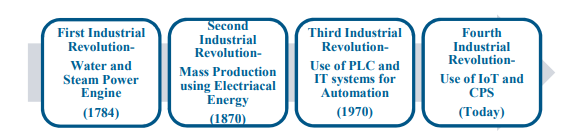
\includegraphics[width=0.8\linewidth]{gambar/industry-40.png}
    \caption{Evolusi industri dunia \cite{industry40}}
    \label{fig:industry40}
\end{figure}

Data adalah output utama dalam implementasi \textit{IoT}. Dimana fungsi \textit{IoT} sebenarnya, dengan bantuan sensor dan konektivitas, adalah untuk mencari informasi melalui data yang didapatkan. Dimana data menjadi alasan terbentuknya informasi yang sempurna jika data tersebut dapat dimanfaatkan dengan baik. Informasi sempurna inilah yang menjadi dasar pentingnya \textit{IoT} pada dunia teknologi, informasi memungkinkan kita untuk mengambil keputusan dan mengatur berdasarkan informasi yang konkrit, sehingga dapat digunakan sebagai acuan untuk melakukan automasi dalam berbagai aspek untuk kehidupan yang lebih efisien. \parencite{iot-sg}

Pada dasarnya arsitektur \textit{IoT} dibagi menjadi 3 bagian, yaitu lapisan \textit{Application, Network, dan Perception} dimana \textit{Application} atau aplikasi menjadi lapisan yang menyajikan data kepada pengguna juga berfungsi sebegai antarmuka dengan sistem IoT, \textit{Network} atau lapisan jaringan menghubunkan perangkat IoT dengan jaringan internet sehingga dapat berkomunikasi dengan perangkat lainnya, dan terakhir adalah \textit{Perception} atau lapisan persepsi bertugas untuk mengumpulkan data dari lingkungan tertentu dengan perangkat fisik melalui sensor dan aktuator.

Namun pada penulisan baru dilakukan abstraksi pada arsitektur dasar dari \textit{IoT} menjadi lima lapisan, lapisan tersebut dibagi menjadi \textit{Business, Application, Service Management, Object Abstraction, dan Objects}. \textit{Objects} atau lapisan objek sama seperti lapisan persepsi yang berfungsi untuk mengambil dan memproses data melalui sensor fisik, kemudian data yang telah diproses dikirim ke lapisan \textit{Object Abstraction} atau lapisan abstraksi objek yang bertugas untuk mengirim data ke lapisan \textit{Service Management} dengan berbagai protokol yang telah ditentukan di awal, baik itu RFID, 3G, \textit{WiFi, Bluetooth},dll. Kemudian lapisan \textit{Service Management} atau manajemen servis menghubungkan servis dengan pihak yang menggunakannya dengan menyamakan nama dan alamat sehingga dapat saling berkomunikasi dengan protokol jaringan. \textit{Application} atau lapisan aplikasi menyediakan servis pada sistem \textit{IoT} pada penggunanya dalam bentuk antarmuka dengan cara yang intuitif sehingga dapat dimengerti dengan mudah oleh manusia. Terakhir adalah lapisan \textit{Business} atau lapisan bisnis, yang mengatur secara keseluruhan sistem \textit{IoT} mulai dari aktivitas dan servis yang disediakan. Lapisan ini juga bertanggungjawab untuk membuat model bisnis, grafik, \textit{flowchart}, dll. sehingga memudahkan analisa dan pengembangan dari sistem \textit{IoT} yang digunakan. \parencite{iot-arab}

% % Contoh penggunaan referensi dari persamaan
% Kemudian menjadi persamaan seperti pada persamaan \ref{eq:FirstLaw}.

% % Contoh pembuatan persamaan
% \begin{equation}
%   % Label referensi dari persamaan yang dibuat
%   \label{eq:FirstLaw}
%   % Baris kode persamaan yang dibuat
%   \sum \mathbf{F} = 0\; \Leftrightarrow\; \frac{\mathrm{d} \mathbf{v} }{\mathrm{d}t} = 0.
% \end{equation}

\subsection{Mikrokontroler ESP32}
ESP32 adalah sebuah mikrkontroler \textit{System on Chip (SOC)} oleh Espressif yang terintegrasi dengan \textit{Wi-Fi} dan \textit{Bluetooth}. ESP32 menggunakan prosesor 40nm Xtensa 32-bit dengan frekuensi 240Mhz, \textit{RAM} sebesar 520KB, dan \textit{ROM} sebesar 448KB. Prosesor yang digunakan ESP32 sangat rendah daya sehingga dapat digunakan dalam proyek dengan ukuran jejak yang kecil yang menggunakan baterai. Kapabilitas Wi-Fi dan Bluetooth dari ESP32 juga memudahkan penggunanya untuk  mengembangkan sistem yang dapat berkomunikasi secara nirkabel. Dalam ranah IoT, ESP32 termasuk ke dalam lapisan objek atau persepsi, dimana ESP32 dapat digunakan sebagai alat fisik yang mengumpulkan data dengan bantuan sensor yang dapat dihubungkan melalui 30 \textit{GPIO (General Purpose Input/Output)} yang ada pada ESP32. Aplikasi dari ESP32 tidak terbatas, dimana dapat diimplementasikan ekdalam sistem otomasi, \textit{Wearable Devices}, sistem sensor jaringan, robotika, dan banyak lagi. \parencite{esp32}

Berikut adalah pin yang tersedia pada ESP32 SoC,

\begin{figure}[H]
    \centering
    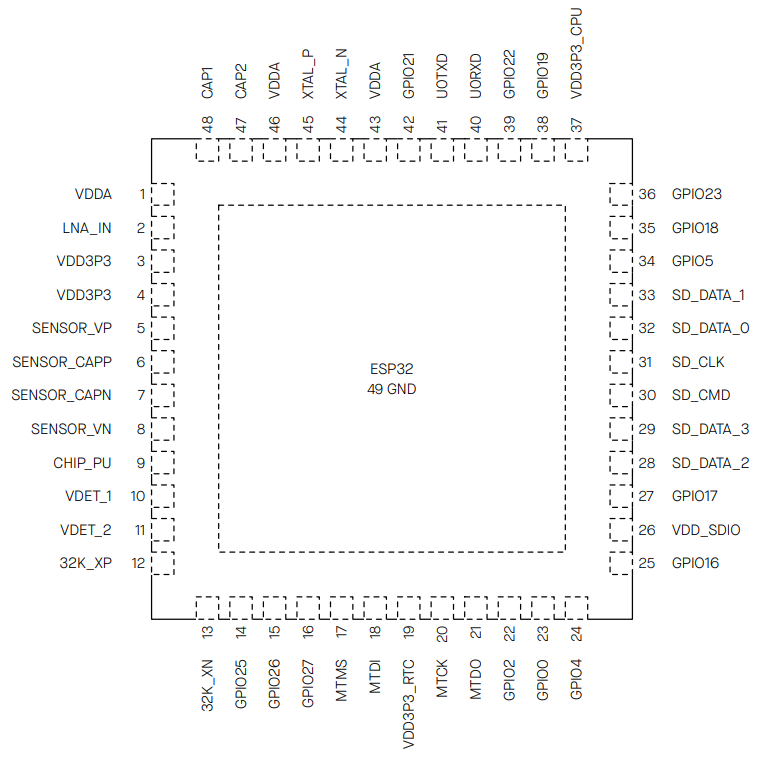
\includegraphics[width=0.45\linewidth]{gambar/pinout-esp32.png}
    \caption{\emph{Pinout} dari SoC ESP32}
    \label{fig:esp-32-pinout}
\end{figure}

Fungsi dari tiap pin bisa lebih dari satu, power pin yang ada pada ESP32 adalah sebagai berikut, dimana Vin adalah pin untuk memberikan daya dengan tegangan 5V - 12V, kemudian pin 3.3V yang digunakan untuk memberikan daya kepada perangkat eksternal, dan GND yang digunakan sebagai ground dari perangkat ESP32.
Ada 40 pin \textit{GPIO} pada ESP32 yang memiliki fungsi yang berbeda - beda. Pin GPIO 0-5 dan 12-33 memiliki fungsi digital input dan output dan pin 34-39 digunakan sebagai input saja, sedangkan pin 6-11 terhubung secara internal dalam ESP32. Beberapa dari pin ini juga memiliki fungsi lain seperti komunikasi UART, I2C, dan PWM juga beberapa pin yang digunakan sebagai \textit{Analog to Digital Converter dan Digital to Analog Converter}. Fungsi - fungsi yang lengkap ini sangat membantu dalam pembuatan proyek yang bervariasi.

Beberapa modul koneksi nirkabel yang dapat diutilisasikan oleh ESP32 adalah Bluetooth dan Wi-Fi. Teknologi Bluetooth yang digunakan pada SoC ESP32 adalah versi 4.2 dengan \textit{bandwidth} maksimum hingga 4 Mbps dan power transmisi sebesar +9 dBm juga sudah dapat terhubung ke lebih dari satu perangkat. Wi-Fi yang terintegrasi dalam ESP32 menggunakan frekuensi di 2.4GHz dengan protokol 802.11b/g/n yang dapat melakukan transmisi data hingga 150 Mbps. Salah satu protokol yang dapat digunakan dengan Bluetooth dan Wi-Fi pada ESP32 adalah protokol ESP-NOW, dimana protokol tersebut memungkinkan komunikasi antara perangkat ESP32 menggunakan daya dan \textit{latency} yang rendah tanpa membutuhkan akses poin atau router. \parencite{esp32-datasheer}

\subsection{\textit{Computer Numerical Control}}
Mesin kontrol numerik adalah mesin yang diatur menggunakan perhitungan numerik untuk menjalankan suatu tujuan tertentu, mesin ini dibagi menjadi dua, yaitu mesin pemotong dan mesin non-pemotong. Mesing pemotong artinya mesing yang menghilangkan materi dari sebuah objek untuk menciptakan suatu bentuk tertentu, contoh dari mesin ini adalah mesin \textit{milling} dan mesin bubut. Sedangkan mesin non-pemotong merubah bentuk dari sebuah objek dengan memberikan gaya kepada objek, contohnya adalah mesin pres. Sistem gerak pada robot juga termasuk kedalam mesin non-pemotong. CNC atau \textit{Computer Numerical Control} adalah sistem atau mesin kontrol numerik yang diatur dengan bantuan perhitungan komputer sehingga dapat dikontrol dengan akurasi dan efisiensi. 

Mesin CNC merubah perhitungan dari sebuah sistem numerik dengan menggunakan me- kanisme penggerak yang digerakkan oleh servo, dimana merupakan sebuah motor yang bergerak pada sebuah \textit{axis} sesuai dengan perintah tertentu, namun pergerakan yang dilakukan oleh motor berbentuk pergerakan rotasi sehingga perlu diubah menjadi gerakan yang linear, ada beberapa cara yang dapat dilakukan untuk mengubah bentuk pergerakan tersebut, yang pertama adalah dengan menggunakan \textit{coupling} dan \textit{ball screw}, seperti pada gambar \ref{fig:nut-screw}, dimana sekrup akan berputar sesuai dengan perputaran motor dan mur yang terletak pada sekrup akan bergerak secara linier. Cara kedua adalah menggunakan sistem \textit{belt dan pulley}, seperti pada gambar \ref{fig:pulley}, yang mengubah pergerakan rotasi dari servo motor menjadi gerakan linier pada sabuk yang terpasang dalam sistem. 

\begin{figure}[H]
    \centering
    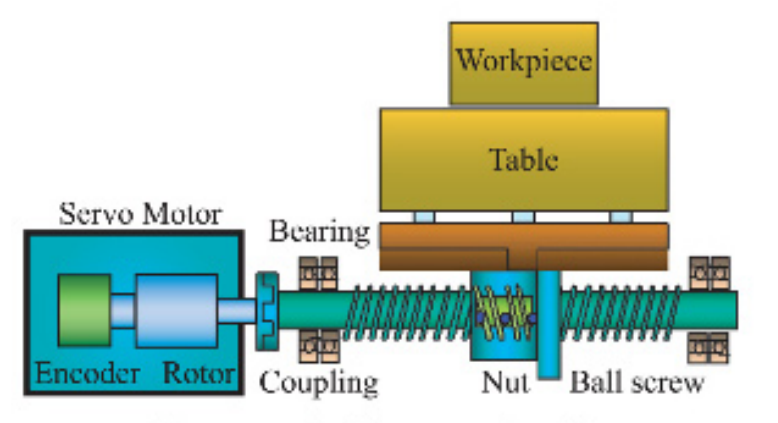
\includegraphics[width=0.5\linewidth]{gambar/nut-screw-mech.png}
    \caption{Sistem gerak linear dengan sekrup dan mur}
    \label{fig:nut-screw}
\end{figure}

\begin{figure}[H]
    \centering
    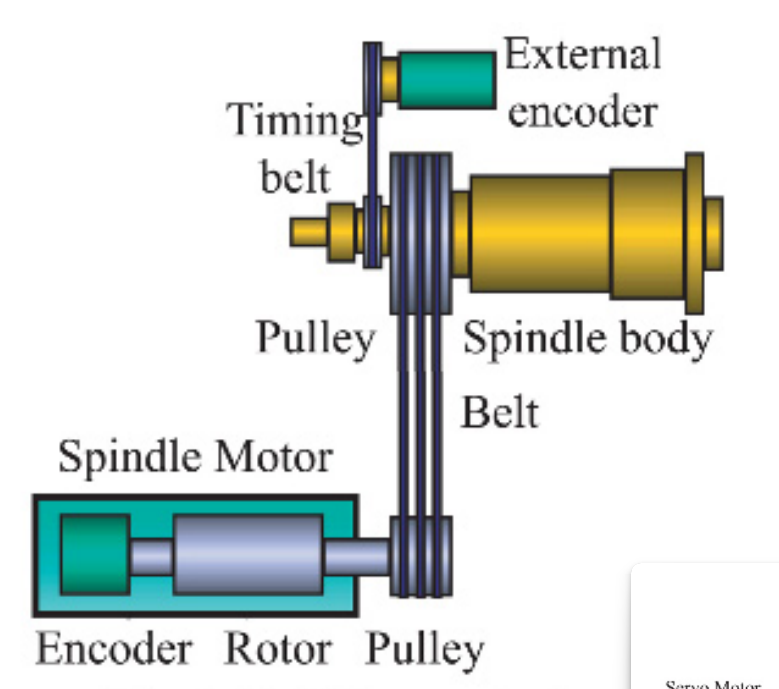
\includegraphics[width=0.4\linewidth]{gambar/pully-mech.png}
    \caption{Sistem gerak liner dengan sistem \textit{belt dan pulley}}
    \label{fig:pulley}
\end{figure}

Ada beberapa jenis yang dapat digunakan sebagai motor penggerak dalam sistem \textit{CNC}, yaitu servo motor DC, servo motor AC sinkronus, dan servo motor AC induksi, sesuai dengan gambar \ref{fig:servo-types}.

\begin{figure}[H]
    \centering
    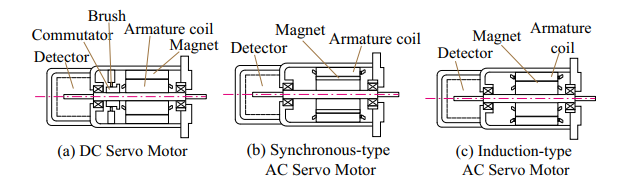
\includegraphics[width=0.8\linewidth]{gambar/servo-motor-diff.png}
    \caption{Tipe - tipe servo motor}
    \label{fig:servo-types}
\end{figure}

Servo motor DC, seperti pada gambar \ref{fig:servo-types}a, merupakan motor yang terbuat dari yang stator terdiri dari bingkai silinder, yang berperan sebagai jalur untuk fluks magnetik dan pendukung mekanis, dan magnet, yang dipasang ke bagian dalam bingkai. Rotor terdiri dari poros dan sikat. Komutator dan rangka penyangga logam rotor (inti rotor) dipasang pada bagian luar poros dan angker dililitkan pada rangka penyangga logam rotor. Sikat yang memasok arus melalui komutator dibuat dengan kumparan jangkar. Di bagian belakang poros, detektor untuk mendeteksi kecepatan rotasi terpasang pada rotor. Servo motor AC sinkronus merupakan servo yang tebuat dari stator yang terdiri dari rangka silinder dan inti stator. Inti stator terletak di dalam rangka dan kumparan jangkar dililitkan di sekitar inti stator. Ujung kumparan dihubungkan dengan kabel utama dan arus disediakan dari kabel utama. Rotor terdiri dari poros dan magnet permanen dan magnet permanen dipasang di bagian luar poros. Pada motor servo AC tipe sinkron, magnet dipasang ke rotor dan kumparan jangkar dililitkan di sekitar stator tidak seperti motor servo DC. Oleh karena itu, suplai arus dimungkinkan dari luar tanpa stator dan motor servo AC tipe sinkron disebut “motor servo \textit{brushless}” karena karakteristik struktural ini. Karena struktur ini memungkinkan untuk mendinginkan inti stator langsung dari luar, maka dimungkinkan untuk menahan peningkatan suhu. Terakhir ada motor servo AC induksi, dimana struktur motor servo AC tipe induksi identik dengan motor induksi pada umumnya. Jika arus bolak-balik multi-fase mengalir melalui kumparan stator, arus diinduksi dalam kumparan rotor dan arus induksi menghasilkan torsi. Pada motor servo AC jenis ini, stator terdiri dari rangka, inti stator, kumparan jangkar, dan kawat timah. Rotor terdiri dari poros dan inti rotor yang dibangun dengan konduktor.

Kemudian dalam sistem CNC juga terdapat enkoder, yaitu perangkat yang mendeteksi posisi saat ini untuk kontrol posisi, umumnya, dibangun di ujung poros transmisi daya. Untuk mengontrol kecepatan, kecepatan dideteksi oleh sensor atau dihitung oleh data kontrol posisi yang terdeteksi dari encoder. Metode untuk mendeteksi kecepatan menggunakan encoder, cara menghitung pulsa yang dihasilkan dalam satuan waktu dan sarana untuk mendeteksi interval antara pulsa bersama. Ada dua macam jenis enkoder, yaitu optikal dan magnetik. Bagian deteksi encoder tipe magnetik berbeda dengan encoder tipe optik, tetapi kedua jenis encoder ini menghasilkan sinyal output dengan cara yang sama.

Kemudian ada \textit{resolver dan speed sensor}, \textit{resolver} adalah detektor sudut dan posisi rotasi dan digunakan sebagai sensor motor. Tidak seperti encoder yang menghasilkan sinyal output dalam format digital, resolver menghasilkan output dalam format analog. \textit{Resolver} terdiri dari stator, rotor, dan trafo rotasi. Kumparan stator dan rotor disusun untuk membuat distribusi fluks magnetik menjadi gelombang sinus sehubungan dengan sudut. \textit{Resolver} memiliki struktur yang mirip dengan motor dan tidak peka terhadap getaran dan guncangan mekanis. Selain itu, karena outputnya adalah sinyal analog, maka transmisi sinyal jarak jauh dan miniaturisasi perangkat dimungkinkan. Namun demikian, sirkuit pemrosesan sinyal rumit dan perangkat ini lebih mahal daripada rotary encoder. Sedangkan \textit{speed sensor} sesuai namanya adalah sensor kecepatan dalam suatu sistem CNC.

Selain motor dan sensor, ada tiga komponen penting lainnya dalam sebuah sistem CNC yaitu \textit{Linear Movement Guide}, \textit{Coupling}, dan \textit{Control Loop}. \textit{Linear Movement Guide} merupakan sebuah kompenen fisik yang digunakan sebagai jalur untuk sistem CNC fungsi dari komponen ini adalah memastikan pergerakan dalam sistem tetap akurat dan baik. \textit{Linear Movement Guide} terdiri dari rel pemandu berbentuk M dan bagian pemindahan. \textit{Bearing} berada di antara rel pemandu dan bagian pemindahan dan pelumas disuplai ke permukaan rel\textit{Linear Movement Guide} untuk mengurangi gesekan saat bagian pemindahan bergerak. Berikut pada gambar \ref{fig:lmg} adalah contoh dari \textit{Linear Movement Guide}.

\begin{figure}[H]
    \centering
    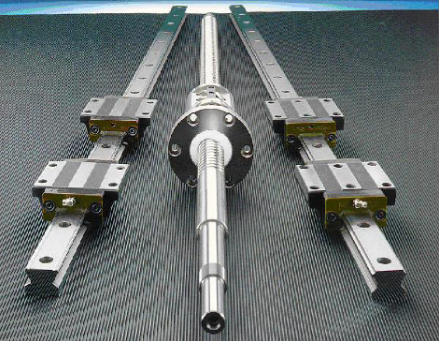
\includegraphics[width=0.6\linewidth]{gambar/lm-gudie.png}
    \caption{\textit{Linear Movement Guide}}
    \label{fig:lmg}
\end{figure}

\textit{Coupling} atau kopling merupakan merupakan salah satu komponen mesin CNC yang menghubungkan poros motor servo dengan sekrup bola. Ketika sekrup bola dan motor servo disambungkan, bagian tengah porosnya harus identik. Namun, dalam praktiknya, ini sangat sulit. Untuk alasan ini, kopling harus dirancang agar tidak sensitif terhadap pusat rotasi yang tidak sejajar. Dan \textit{Control Loop} merupakan rangakaian kontrol yang dilakukan terhadap mesin CNC, kontrol ini dilakukan secara kontinius sehingga pergerakan yang dilakukan oleh mesin CNC akurat. Kontrol ini dapat dilakukan dengan akurat dengan menggunakan sensor dan motor yang menjadi komponen utama dari CNC.

Sistem CNC dapat diatur dengan menggunakan instruksi yang diberikan secara program, instruksi ini dinamakan sebagai \textit{G-Code} yang disiapkan sebelum mesin CNC berfungsi. Kode ini berisi lintasan, kecepatan, dan posisi alat dalam koordinat X, Y, dan Z. Kontrol yang sudah terprogram tersebut akan dioperasikan kepada \textit{Driving Motor} dan sensor pada sistem \textit{CNC}. \parencite{cnc}

\subsection{\textcolor{red}{\textit{3D Modelling} dan \textit{Computer Assisted Design (CAD)}}}

\lipsum[15]

\subsection{Manufaktur Aditif (\textit{3D Printing})}
Manufaktur aditif adalah istilah formal untuk apa yang sering disebut sebagai pembuatan \textit{Rapid Prototyping} dan \textit{3D Printing}. \textit{Rapid prototyping (RP)} adalah proses untuk membuat representasi sistem atau bagian dengan cepat sebelum dirilis atau dikomersialkan. Dengan kata lain, penekanannya adalah menciptakan sesuatu dengan cepat dan hasilnya adalah prototipe atau model dasar yang akan menjadi model selanjutnya dan pada akhirnya menjadi produk. Konsep dari manufaktur aditif dapat direalisasikan dengan memanfaatkan \textit{layering} atau pembuatan komponen adalah penggunaan lapisan - lapisan 2-dimensi dari perpotongan model 3D yang saling ditumpuk. Hampir setiap teknologi manufaktur aditif membuat komponen menggunakan lapisan material yang ditambahkan bersama-sama seperti ini.

Aplikasi dari manufaktur aditif mulai digunakan karena alasan menciptakan visualisasi dari sebuah produk yang sedang dikembangkan karena model fisik yang diciptakan dapat lebih mudah untuk dipahami dibanding gambaran 2-dimensi atau \textit{rendering} 3-dimensi pada umumnya. Semakin meningkatnya kualitas dari hasil manufaktur aditif, baik dari aspek akurasi, material, dan kecepatan, hasil dari manufaktur aditif digunakan untuk menguji coba tiga kriteria pada sebuah produk, yaitu \textit{Form, Fit, dan Function}. \textit{Form} adalah sebuah kriteria yang memastikan model yang dihasilkan sesuai dengan bentuk dan kegunaan dari produk, kemudian ada \textit{Fit} yaitu sebuah kriteria yang menjelaskan apakah komponen yang dihasilkan memiliki akurasi dan toleransi yang cukup jika digunakan untuk perakitan produk. Terakhir adalah kriteria \textit{Function} dimana ciri material dan fungsi dari produk dapat digunakan sesuai dengan desain akhir dan tujuan dari produk tersebut.

Prinsip dasar dari teknologi ini adalah bahwa sebuah model, yang awalnya dibuat dengan menggunakan sistem \textit{Computer-Aided Design} (CAD) tiga dimensi, dapat difabrikasi secara langsung tanpa memerlukan perencanaan proses. Meskipun pada kenyataannya tidak sesederhana kedengarannya, teknologi manufaktur aditif tentu saja secara signifikan menyederhanakan proses produksi objek 3D yang kompleks secara langsung dari data CAD. Proses manufaktur lainnya memerlukan analisis yang cermat dan terperinci dari geometri bagian untuk menentukan hal-hal seperti urutan fitur yang berbeda yang dapat dibuat, alat dan proses apa yang harus digunakan, dan perlengkapan tambahan apa yang mungkin diperlukan untuk menyelesaikan bagian tersebut. Sebaliknya, manufaktur aditif hanya membutuhkan beberapa detail dimensi dasar dan sedikit pemahaman tentang cara kerja mesin manufaktur aditif dan bahan yang digunakan untuk membuat komponen. Kunci dari cara kerja manufaktur aditif adalah bahwa komponen dibuat dengan menambahkan material secara berlapis-lapis; setiap lapisan merupakan penampang tipis dari komponen yang berasal dari data CAD asli. Tentunya dalam dunia fisik, setiap lapisan harus memiliki ketebalan yang terbatas sehingga bagian yang dihasilkan akan menjadi perkiraan dari data asli, seperti yang diilustrasikan oleh gambar \ref{fig:cad}. Semakin tipis setiap lapisan, semakin dekat bagian akhir dengan aslinya. Semua mesin manufaktur aditif yang dikomersialkan hingga saat ini menggunakan pendekatan berbasis lapisan, dan perbedaan utamanya terletak pada bahan yang dapat digunakan, bagaimana lapisan dibuat, dan bagaimana lapisan diikat satu sama lain. Perbedaan tersebut akan menentukan faktor-faktor seperti keakuratan bagian akhir serta sifat material dan sifat mekanisnya. Perbedaan tersebut juga akan menentukan faktor-faktor seperti seberapa cepat komponen dapat dibuat, berapa banyak pasca-pemrosesan yang diperlukan, ukuran mesin manufaktur aditif yang digunakan, dan biaya keseluruhan mesin dan proses.

\begin{figure}[H]
    \centering
    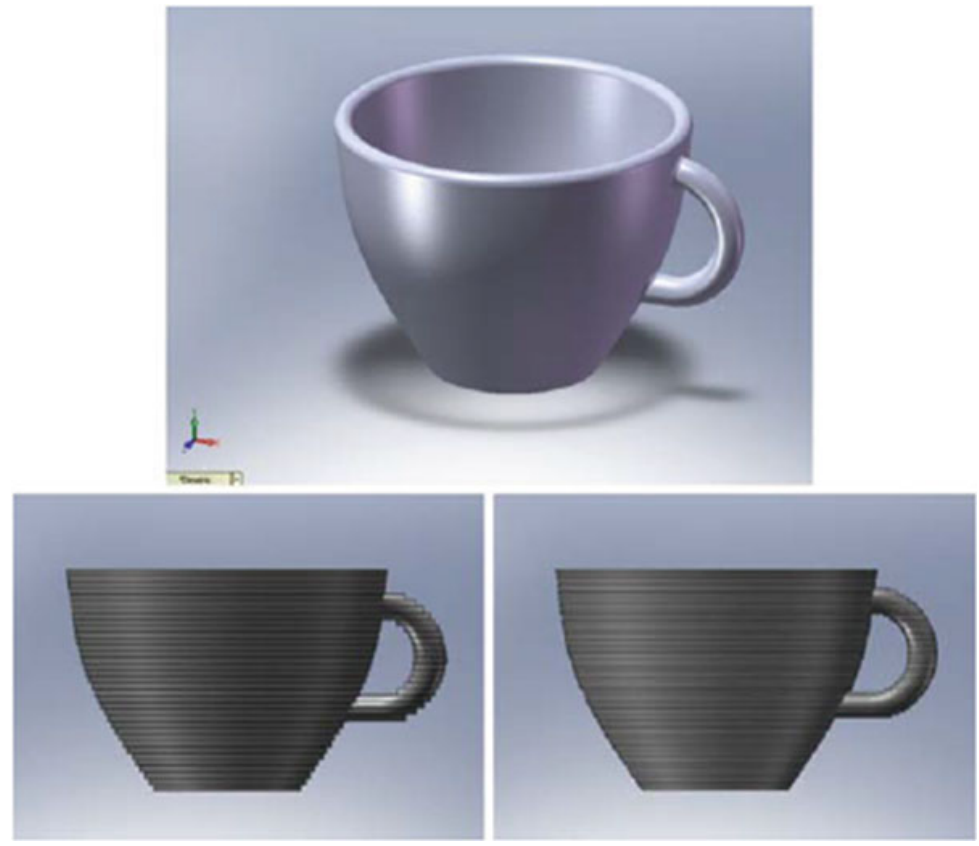
\includegraphics[width=0.6\linewidth]{gambar/cad-image.png}
    \caption{Rendering tiga dimensi dengan menggunakan \textit{Computer Aided Design}}
    \label{fig:cad}
\end{figure}

Seperti yang sudah dijelaskan diatas, manufaktur aditif secara keseluruhan menggunakan pendekatan sama yaitu dengan berbasis lapisan, namun dapat diklasifikasikan sesuai dengan teknologi yang digunakan untuk menghasilkan tiap lapisan tersebut. Jenis dari manufaktur aditif sangat banyak, namun pada umunya yang sering digunakan adalah \textit{SLA, SLS, dan FDM}. \textit{SLA atau Stereolithography} atau yang disebut juga sebagai \textit{Vat Photpolymerisation} adalah salah satu bentuk dari manufaktur aditif yang memanfaatkan sinar laser ultraviolet yang dapat menyebabkan material tertentu (seperti resin) berubah menjadi sebuah polymer yang mengeras sehingga menghasilkan sebuah objek 3-dimensi. \textit{SLS} atau \textit{Selective Laser Sintering} juga sebuah teknik manufaktur aditif yang menggunakan laser, namun laser yang digunakan merupakan laser dengan suhu tinggi yang dapat menyebabkan material tertentu (nilon atau polyamida) yang awalnya berbentuk bubuk, saling mengikat satu sama lain karna suhu tinggi tersebut sehingga dapat mengeras yang dilakukan dari tiap lapisan - lapisan dengan tinggi tertentu dan menghasilkan sebuah objek. Terakhir adalah \textit{FDM} atau \textit{Fused Deposition Modelling} adalah teknik manufaktur aditif yang menggunakan bahan plastik yang dipanaskan pada suhu tertentu (sesuai dengan jenis plastik yang digunakan) untuk menghasilkan sebuah bentuk tertentu, kemudian berbagi bentuk - bentuk ini ditumpuk sehingga menghasilkan barang 3-dimensi.

Berikut adalah beberapa contoh dari alat - alat manufaktur aditif

\begin{figure}[H]
    \centering
    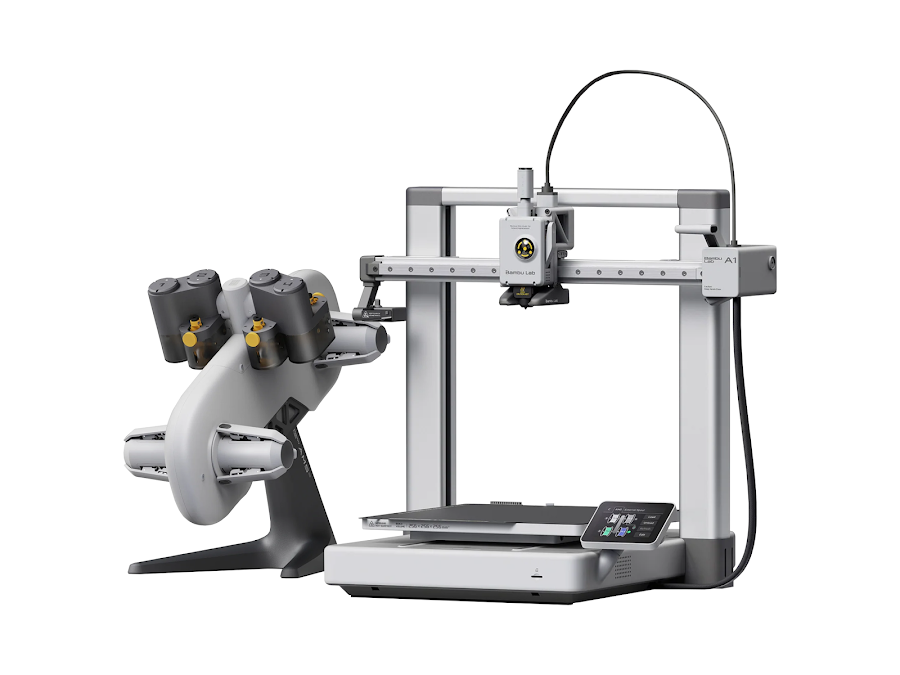
\includegraphics[width=0.35\linewidth]{gambar/fdm-3d-printer.png}
    \caption{Alat 3D Printer dengan Teknologi FDM \textit{(Fused Deposition Modelling)}}
    \label{fig:fdm-3d-printer}
\end{figure}

\begin{figure}[H]
    \centering
    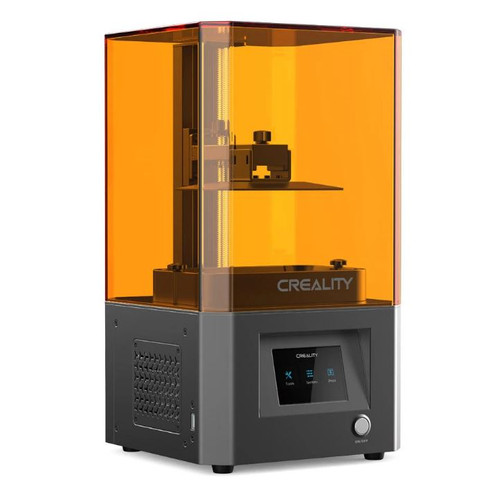
\includegraphics[width=0.25\linewidth]{gambar/sla-3d-printer.jpg}
    \caption{Alat 3D Printer dengan Teknologi SLA \textit{(Stereolithography)}}
    \label{fig:sla-3d-printer}
\end{figure}

\begin{figure}[H]
    \centering
    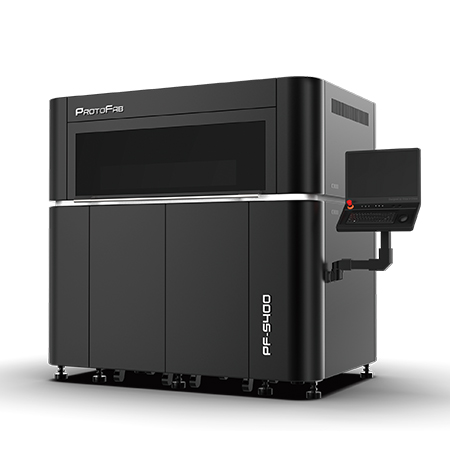
\includegraphics[width=0.3\linewidth]{gambar/sls-3d-printer.jpg}
    \caption{Alat 3D Printer dengan Teknologi SLS \textit{(Selective Laser Sintering)}}
    \label{fig:sls-3d-printer}
\end{figure}

Secara luas manufaktur aditif memiliki banyak kesamaan dengan teknologi mesin CNC. Dimana merupakan sebuah alat yang menghasilkan produk menggunakan bantuan komputer. Perbedaan utama dari kedua teknik ini adalah teknik yang digunakan dimana alat CNC utamanya menggunakan teknik subtraktif yang membutuhkan sebuah blok material tertentu untuk menghasilkan sebuah produk dengan desain yang telah ditentukan. Namun ada beberapa hal lainnya yang lebih rinci yang dapat membedakan kedua teknik manufaktur ini, yaitu material, kecepatan, kompleksitas, akurasi, geometri, dan pemrograman. Secara material teknologi manufaktur aditif pada awalnya dikembangkan di sekitar bahan polimer, lilin, dan laminasi kertas. Selanjutnya, diperkenalkan bahan komposit, logam, dan keramik. Pemesinan CNC dapat digunakan untuk bahan lunak, seperti papan serat kepadatan menengah (MDF), busa yang dapat dikerjakan dengan mesin, lilin yang dapat dikerjakan dengan mesin, dan bahkan beberapa polimer. Secara kecepatan, Pemesinan CNC pada umumnya dapat membuang material jauh lebih cepat daripada mesin manufaktur aditif dapat menambahkan volume material yang sama. Namun, ini hanya sebagian dari gambaran, karena teknologi manufaktur aditif dapat digunakan untuk memproduksi komponen dalam satu tahap. Mesin CNC memerlukan penyiapan dan perencanaan proses yang cukup banyak, terutama karena komponen menjadi lebih kompleks dalam geometrinya. Secara kompleksitas, semakin tinggi kompleksitas geometris, semakin besar keunggulan teknik manufaktur aditif dibandingkan CNC. Jika CNC digunakan untuk membuat bagian secara langsung dalam satu bagian, maka mungkin ada beberapa fitur geometris yang tidak dapat dibuat. Karena alat pemesinan harus dibawa dalam spindel, mungkin ada kendala aksesibilitas atau benturan tertentu yang mencegah alat tersebut ditempatkan pada permukaan pemesinan suatu bagian. Proses AM tidak dibatasi dengan cara yang sama dan \textit{undercut} serta fitur internal dapat dengan mudah dibuat secara mudah tanpa perencanaan proses yang spesifik. Bagian-bagian tertentu tidak dapat dibuat dengan CNC kecuali jika dipecah menjadi beberapa komponen dan dipasang kembali pada tahap selanjutnya. Secara akurasi, mesin manufaktur aditif pada umumnya beroperasi dengan resolusi beberapa puluh mikron. Biasanya mesin AM juga memiliki resolusi yang berbeda di sepanjang sumbu ortogonal yang berbeda. Biasanya, sumbu build vertikal sesuai dengan ketebalan lapisan dan ini akan memiliki resolusi yang lebih rendah dibandingkan dengan dua sumbu pada \textit{build plate}.  Sedangkan akurasi pada mesin CNC, utamanya ditentukan oleh resolusi pemosisian yang serupa di sepanjang ketiga sumbu ortogonal dan oleh diameter alat potong putar. Ada beberapa faktor yang ditentukan oleh geometri pahat, seperti jari-jari sudut internal, tetapi ketebalan dinding bisa lebih tipis daripada diameter pahat karena ini adalah proses subtraktif. Dalam kedua kasus tersebut, detail yang sangat halus juga akan menjadi fungsi dari geometri dan sifat material yang diinginkan. Secara geometri, mesin manufaktur aditif pada dasarnya memecah masalah 3D yang rumit menjadi serangkaian penampang 2D sederhana dengan ketebalan nominal. Dengan cara ini, koneksi permukaan dalam 3D dihilangkan dan kontinuitas ditentukan oleh seberapa dekat kedekatan satu penampang dengan penampang yang berdekatan. Karena hal ini tidak dapat dengan mudah dilakukan dalam CNC, pemesinan permukaan biasanya harus dibuat dalam ruang 3D. Terakhir secara pemrograman, urutan pemgoraman untuk mesin CNC bisa sangat rumit, termasuk pemilihan pahat, pengaturan kecepatan mesin, posisi dan sudut pendekatan, dll. Banyak mesin manufaktur aditif juga memiliki opsi yang harus dipilih, tetapi kisaran, kerumitan, dan implikasi seputar pilihannya sangat minim jika dibandingkan. \parencite{3dprinting}

\subsection{Meteran Listrik Prabayar}
Meteran Listrik Prabayar atau yang disebut sebagai Listrik Pintar, sesuai gambar \ref{fig:meteran-prabayar} merupakan alat yang dikeluarkan oleh PT. PLN dimana pembayaran listrik yang awalnya dilakukan diakhir pemakaian dan dihitung oleh PLN sekarang dilakukan dengan mengisi token secara prabayar sehingga pengguna bisa mengatur seberapa banyak listrik yang digunakan dengan lebih mudah.

\begin{figure}[H]
    \centering
    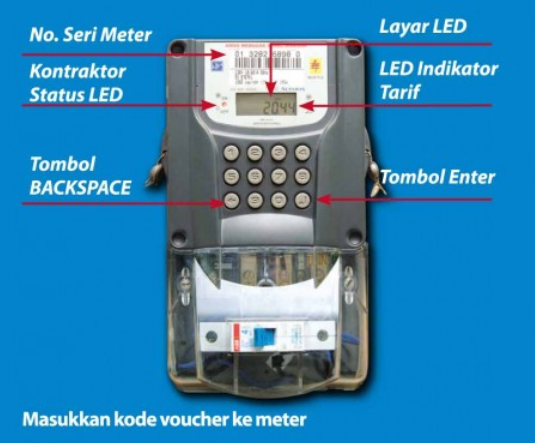
\includegraphics[width=0.5\linewidth]{gambar/meteran-prabayar.png}
    \caption{Meteran listrik prabayar PLN}
    \label{fig:meteran-prabayar}
\end{figure}

Mengisi token dapat dilakukan dengan cara membeli token melalui gerai ATM atau melalui loket pembayaran tagihan listrik online lainnya. Token atau pulsa listrik ini terdiri dari 20 digit angka yang dimasukkan kedalam kWh meteran khusus dari PLN. Token ini setelah dimasukkan akan berbentuk kWh yang dapat dilihat di meteran listrik dengan nilai yang telah ditentukan ketika membeli token.

Beberapa kelebihan yang dimiliki meteran listrik prabayar dibanding meteran tradisional ini adalah kemudahan untuk membeli token, monitoring dari meteran listrik yang lebih mudah, dan dapat privasi yang lebih terjaga. Dan jika energi listrik yang tersimpan di meteran sudah hampir habis, maka meteran akan memberikan sinyal awal suara agar segera dapat dilakukan pengisian ulang.
  \cleardoublepage

  % Konten metodologi
  \chapter{METODOLOGI}

% Ubah konten-konten berikut sesuai dengan isi dari metodologi
Berikut, pada gambar \ref{fig:blok-diagram}, adalah blok diagram dari penelitian yang dilakukan, 
yang secara besar terdiri dari 5 tahap.

\begin{figure}[H]
    \centering
    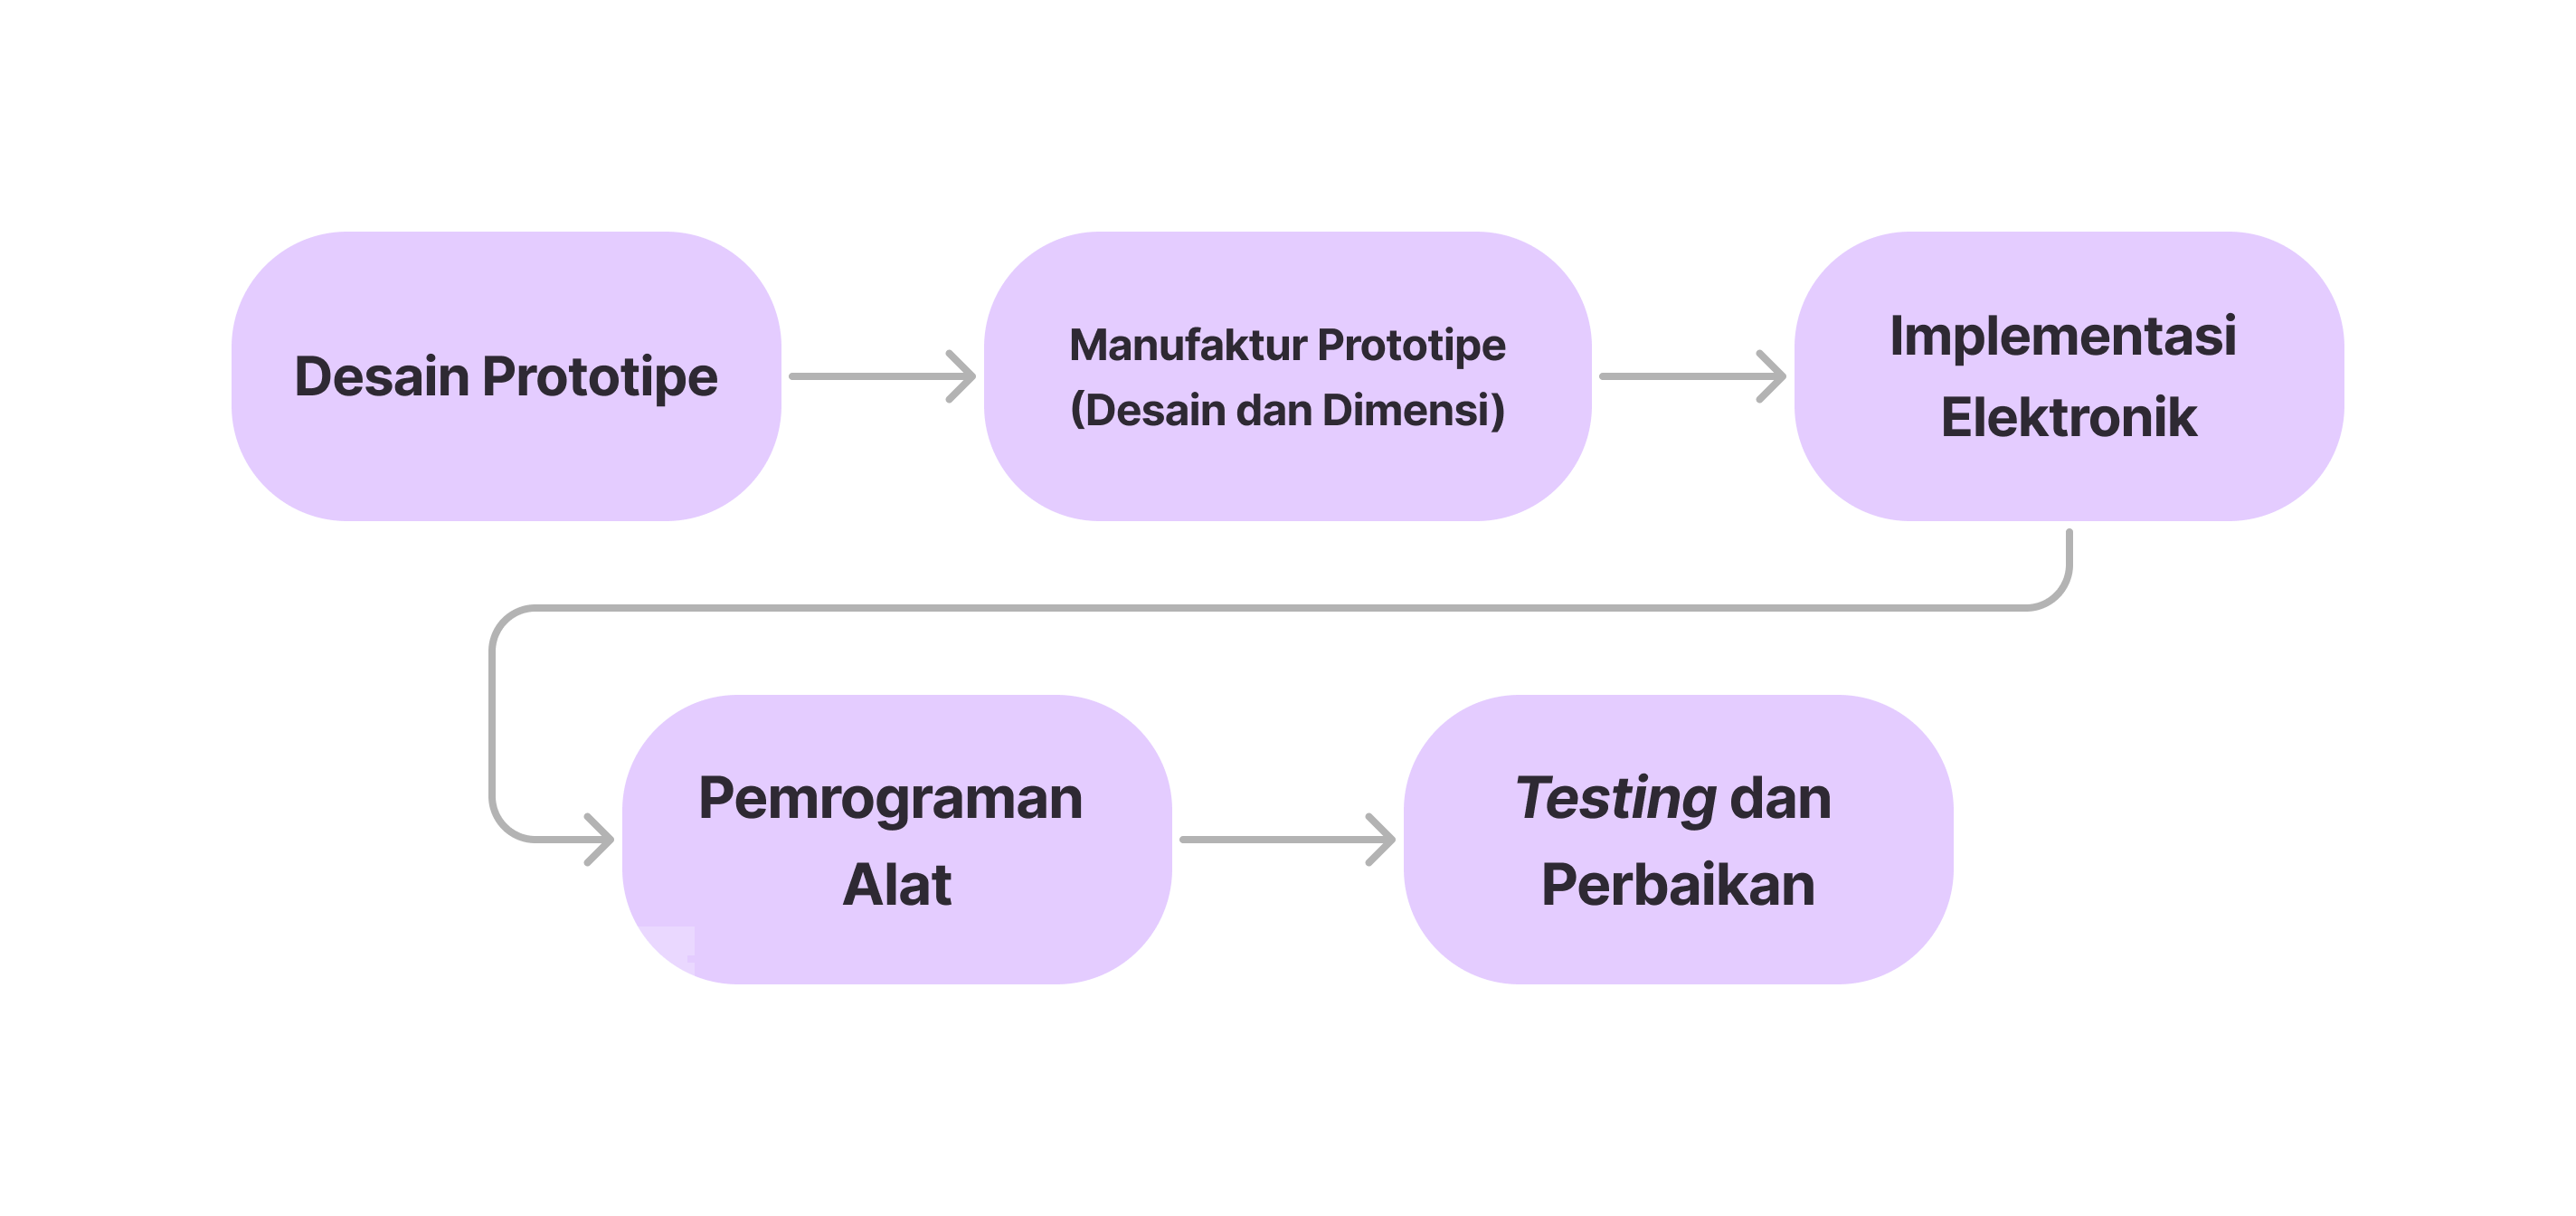
\includegraphics[width=1\linewidth]{gambar/diagram-metodologi.png}
    \caption{Blok Diagram Penelitian}
    \label{fig:blok-diagram}
\end{figure}

\section{Desain Prototipe}

Desain diawali dengan menggambar kasaran secara digital menggunakan \textit{software Goodnotes}
pada \textit{iPad}, memastikan desain yang akan dibuat sesuai dengan kebutuhan, fungsionalitas yang diinginkan,
dan ukuran yang sesuai.
Desain prototipe kemudian dilanjutkan dalam bentuk 3D \textit{Modelling} dengan 
bantuan \textit{software Computer Assisted Design} atau yang sering disebut 
sebagai \textit{CAD}. Aplikasi yang akan penulis gunakan dalam penelitian ini 
adalah \textit{Autodesk Fusion 360}. Dengan \textit{software} ini, penulis dapat menghasilkan gambar
teknik yang lebih rinci dan detail, sehingga dapat dijadikan acuan dalam proses manufaktur.
Juga software ini dapat melakukan export file dalam format \textit{.stl} yang dapat digunakan
dalam proses manufaktur menggunakan \textit{3D Printer}.

Ada beberapa desain yang telah dibuat, sesuai pada gambar \ref{fig:desain-prototipe-2} dan gambar 
\ref{fig:desain-prototipe-3}, desain ini dibuat sehingga dapat 
menyesuaikan dengan meteran listrik prabayar yang biasa terpasang di rumah-rumah secara 
\textit{universal}. Dengan desain yang menggunakan \textit{clamp} sehingga dapat menyesuaikan dengan
ukuran alat meteran listrik prabayar yang berbeda-beda.

\begin{figure}[H]
    \centering
    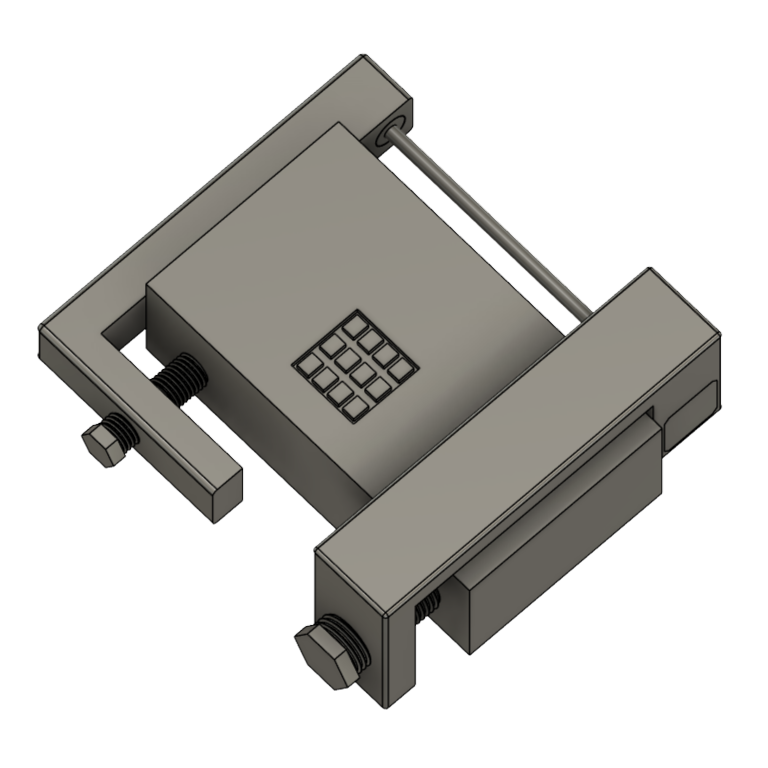
\includegraphics[width=0.4\linewidth]{gambar/prototype-2.png}
    \caption{Desain Prototipe Pertama}
    \label{fig:desain-prototipe-2}
\end{figure}

\begin{figure}[H]
  \centering
  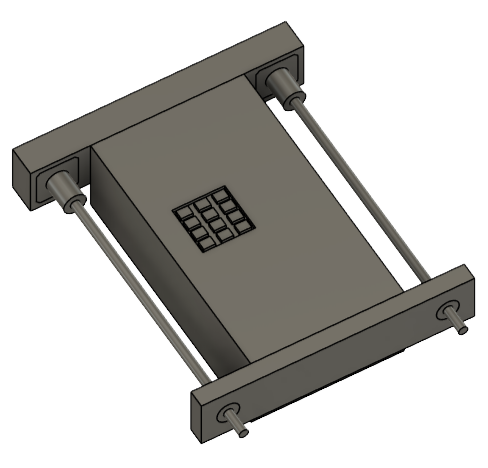
\includegraphics[width=0.4\linewidth]{gambar/prototype-3.png}
  \caption{Desain Prototipe Kedua}
  \label{fig:desain-prototipe-3}
\end{figure}

Desain diatas merupakan protipe yang belum final, dimana masih memerlukan beberapa perbaikan, 
juga bagian pergerakan horizontal (sumbu-x) masih belum diimplementasikan.

\section{Manufaktur Prototipe}

Manufaktur prototipe dilakukan menggunakan bantuan \textit{3D Printer} dengan merek 
\textit{Bambulab A1}. Penulis menggunakan \textit{3D Printer} ini karena dilengkapi dengan fitur yang
sangat lengkap, beberapa dari fitur tersebut adalah
sistem \textit{AMS Lite} yaitu merupakan sistem yang dapat mengatur perubahan material yang digunakan
secara lebih mudah sehingga dapat menggabungkan beberapa material atau warna yang berbeda dalam satu cetakan,
kemudian ada fitur \textit{Auto Bed Leveling} yang dapat mengatur keseimbangan \textit{bed plate} 
dari \textit{3D Printer} secara otomatis memastikan cetakan yang dihasilkan lebih rata dan presisi.
Fitur lainnya yang sangat membantu dalam manufaktur adalah beberapa sensor yang terpasang pada \textit{3D Printer},
beberapanya adalah sensor \textit{filament runout} yang dapat memberikan notifikasi ketika \textit{filament},
habis, kemudian sensor \textit{filament tangle} yang dapat memberikan notifikasi ketika \textit{filament}
terjebak atau terlilit, dan masih banyak lagi fitur lainnya.
Fitur - fitur tersebut sangat membantu dalam proses manufaktur prototipe yang butuh pengulangan
yang cukup banyak, sehingga penulis dapat memfokuskan waktu pada tahap desain dan pengujian.

Proses manufaktur diawali dengan menghasilkan file \textit{.stl} dari desain yang telah dibuat menggunakan \textit{Autodesk Fusion 360}, ke- mudian
file tersebut diolah menggunakan \textit{software Slicer}, sesuai pada gambar \ref{fig:bambu-studio},
yang memotong model 3D menjadi beberapa lapisan dan menyatakan perintah sehingga dapat dicetak oleh \textit{3D Printer}. 
Penulis menggunakan \textit{software Bambu Studio} yang dapat diakses melalui \textit{cloud} yang 
terhubung dengan \textit{3D Printer}. File \textit{.stl} tersebut merupakan representasi dari objek 3 dimensi yang dibuat dari lapisan-lapisan
2 dimensi, yang dimana dijadikan sebagai acuan sesuai dengan lokasi tertentu oleh \textit{3D Printer} 
untuk mencetak objek tersebut. Kemudian file tersebut diunggah ke \textit{cloud} yang terhubung dengan
\textit{3D Printer}, kemudian \textit{3D Printer} akan membaca file tersebut dan mencetak objek tersebut.

\begin{figure}[H]
  \centering
  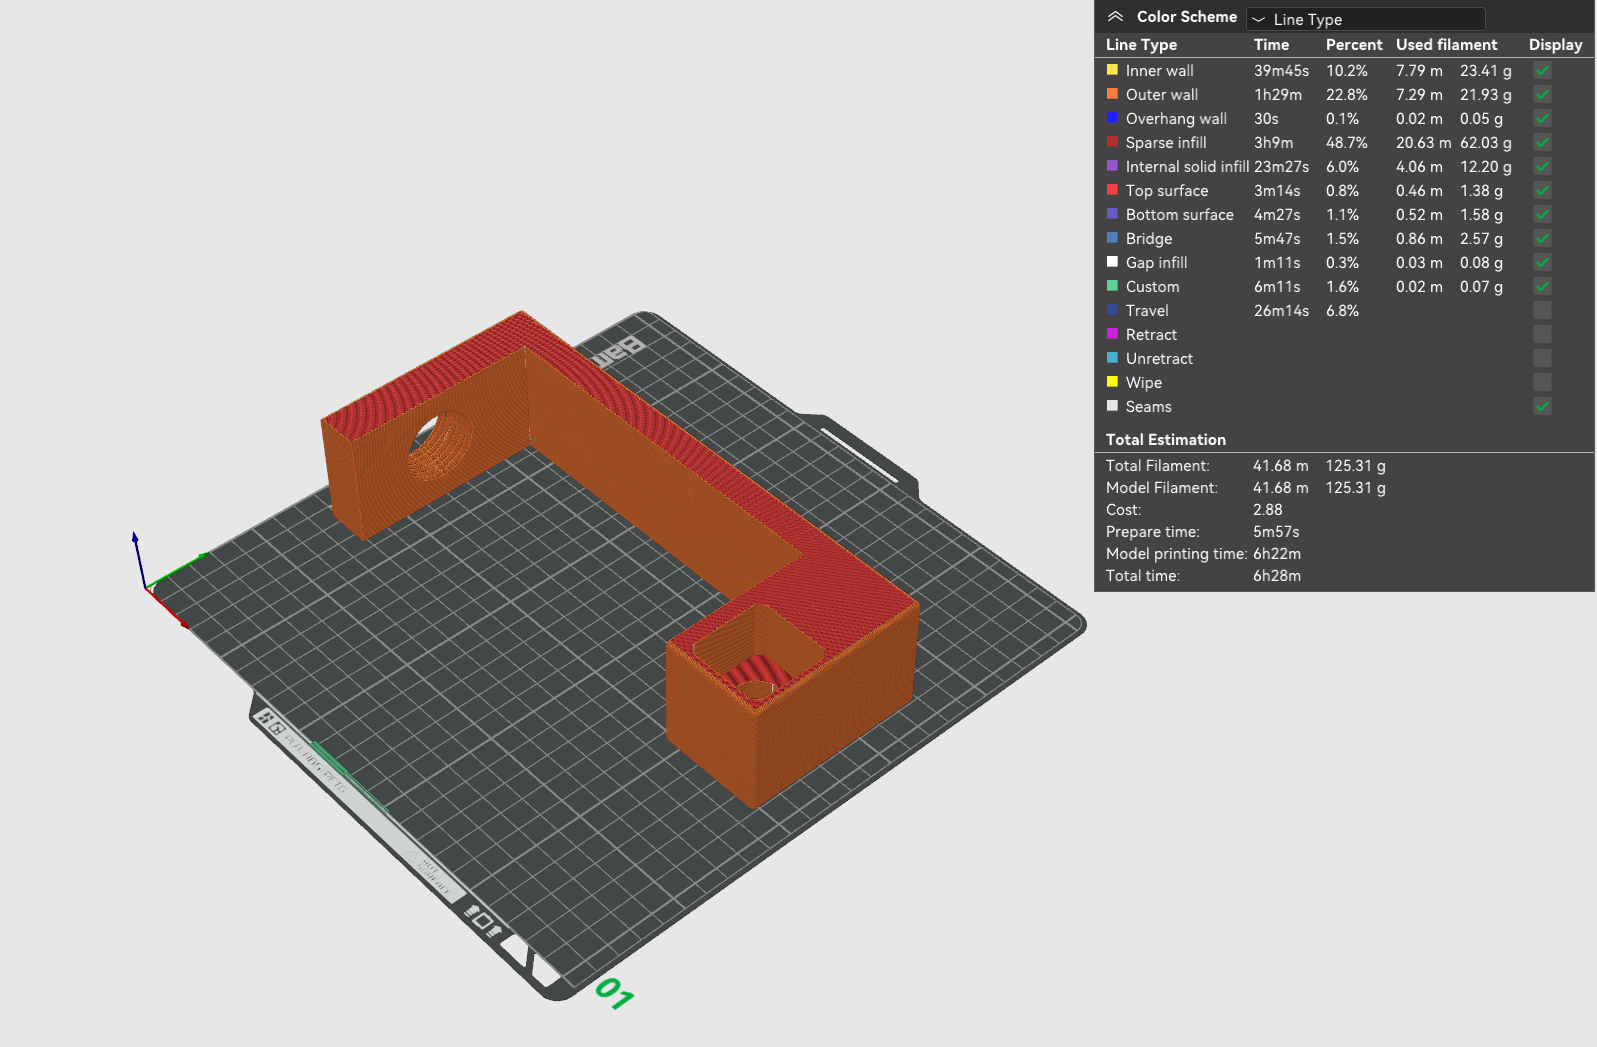
\includegraphics[width=0.7\linewidth]{gambar/bambu-studio.png}
  \caption{file \textit{.stl} yang diolah menggunakan \textit{software Slicer}}
  \label{fig:bambu-studio}
\end{figure}

Hasil dari manufaktur prototipe dan implementasinya tertera pada gambar \ref{fig:hasil-prototipe-1}, dimana prototipe tersebut masih dalam tahap pengujian 
dan perbaikan, namun dapat menjadi visualisasi dan representasi yang baik untuk hasil produk akhir. Material yang digunakan dalam manufaktur prototipe adalah \textit{PLA} atau \textit{Polylactic Acid},
material ini digunakan karena harga nya yang terjangkau, mudah dicetak, dan cukup kuat untuk digunakan
sebagai prototipe. Namun, material ini memiliki kekurangan yaitu tidak tahan terhadap panas dan
suhu tinggi, sehingga tidak dapat digunakan dalam lingkungan yang memiliki suhu tinggi. Sebagai 
alternatif material yang digunakan adalah \textit{PETG} atau \textit{Polyethylene Terephthalate Glycol},
material ini memiliki kelebihan yaitu tahan terhadap suhu tinggi, kuat, dan tahan terhadap benturan,
namun material ini memiliki harga yang lebih mahal dibandingkan \textit{PLA} dan lebih sulit untuk
dicetak.

\begin{figure}[H]
  \centering
  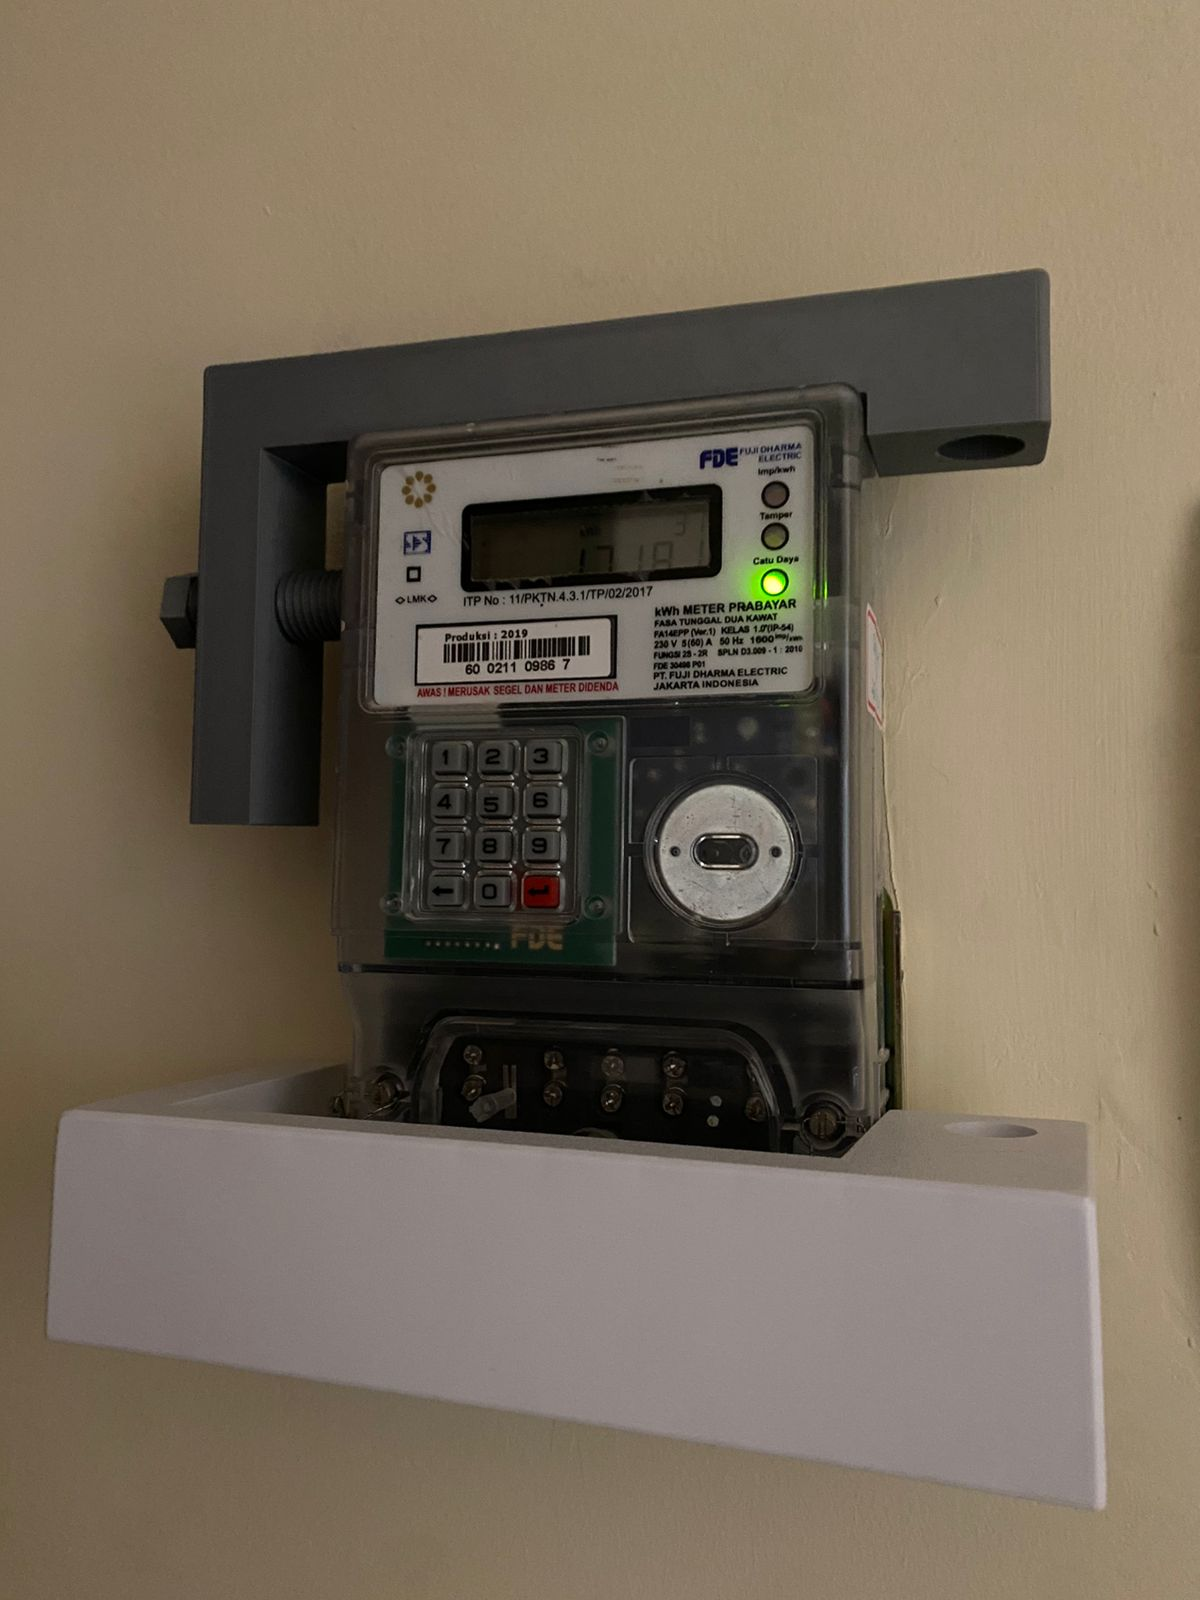
\includegraphics[width=0.4\linewidth]{gambar/contoh-prototipe-kerangka.jpg}
  \caption{Contoh manufaktur prototipe menggunakan \textit{3D Printer}}
  \label{fig:hasil-prototipe-1}
\end{figure}

\section{Implementasi Elektronik}

\begin{figure}[H]
  \centering
  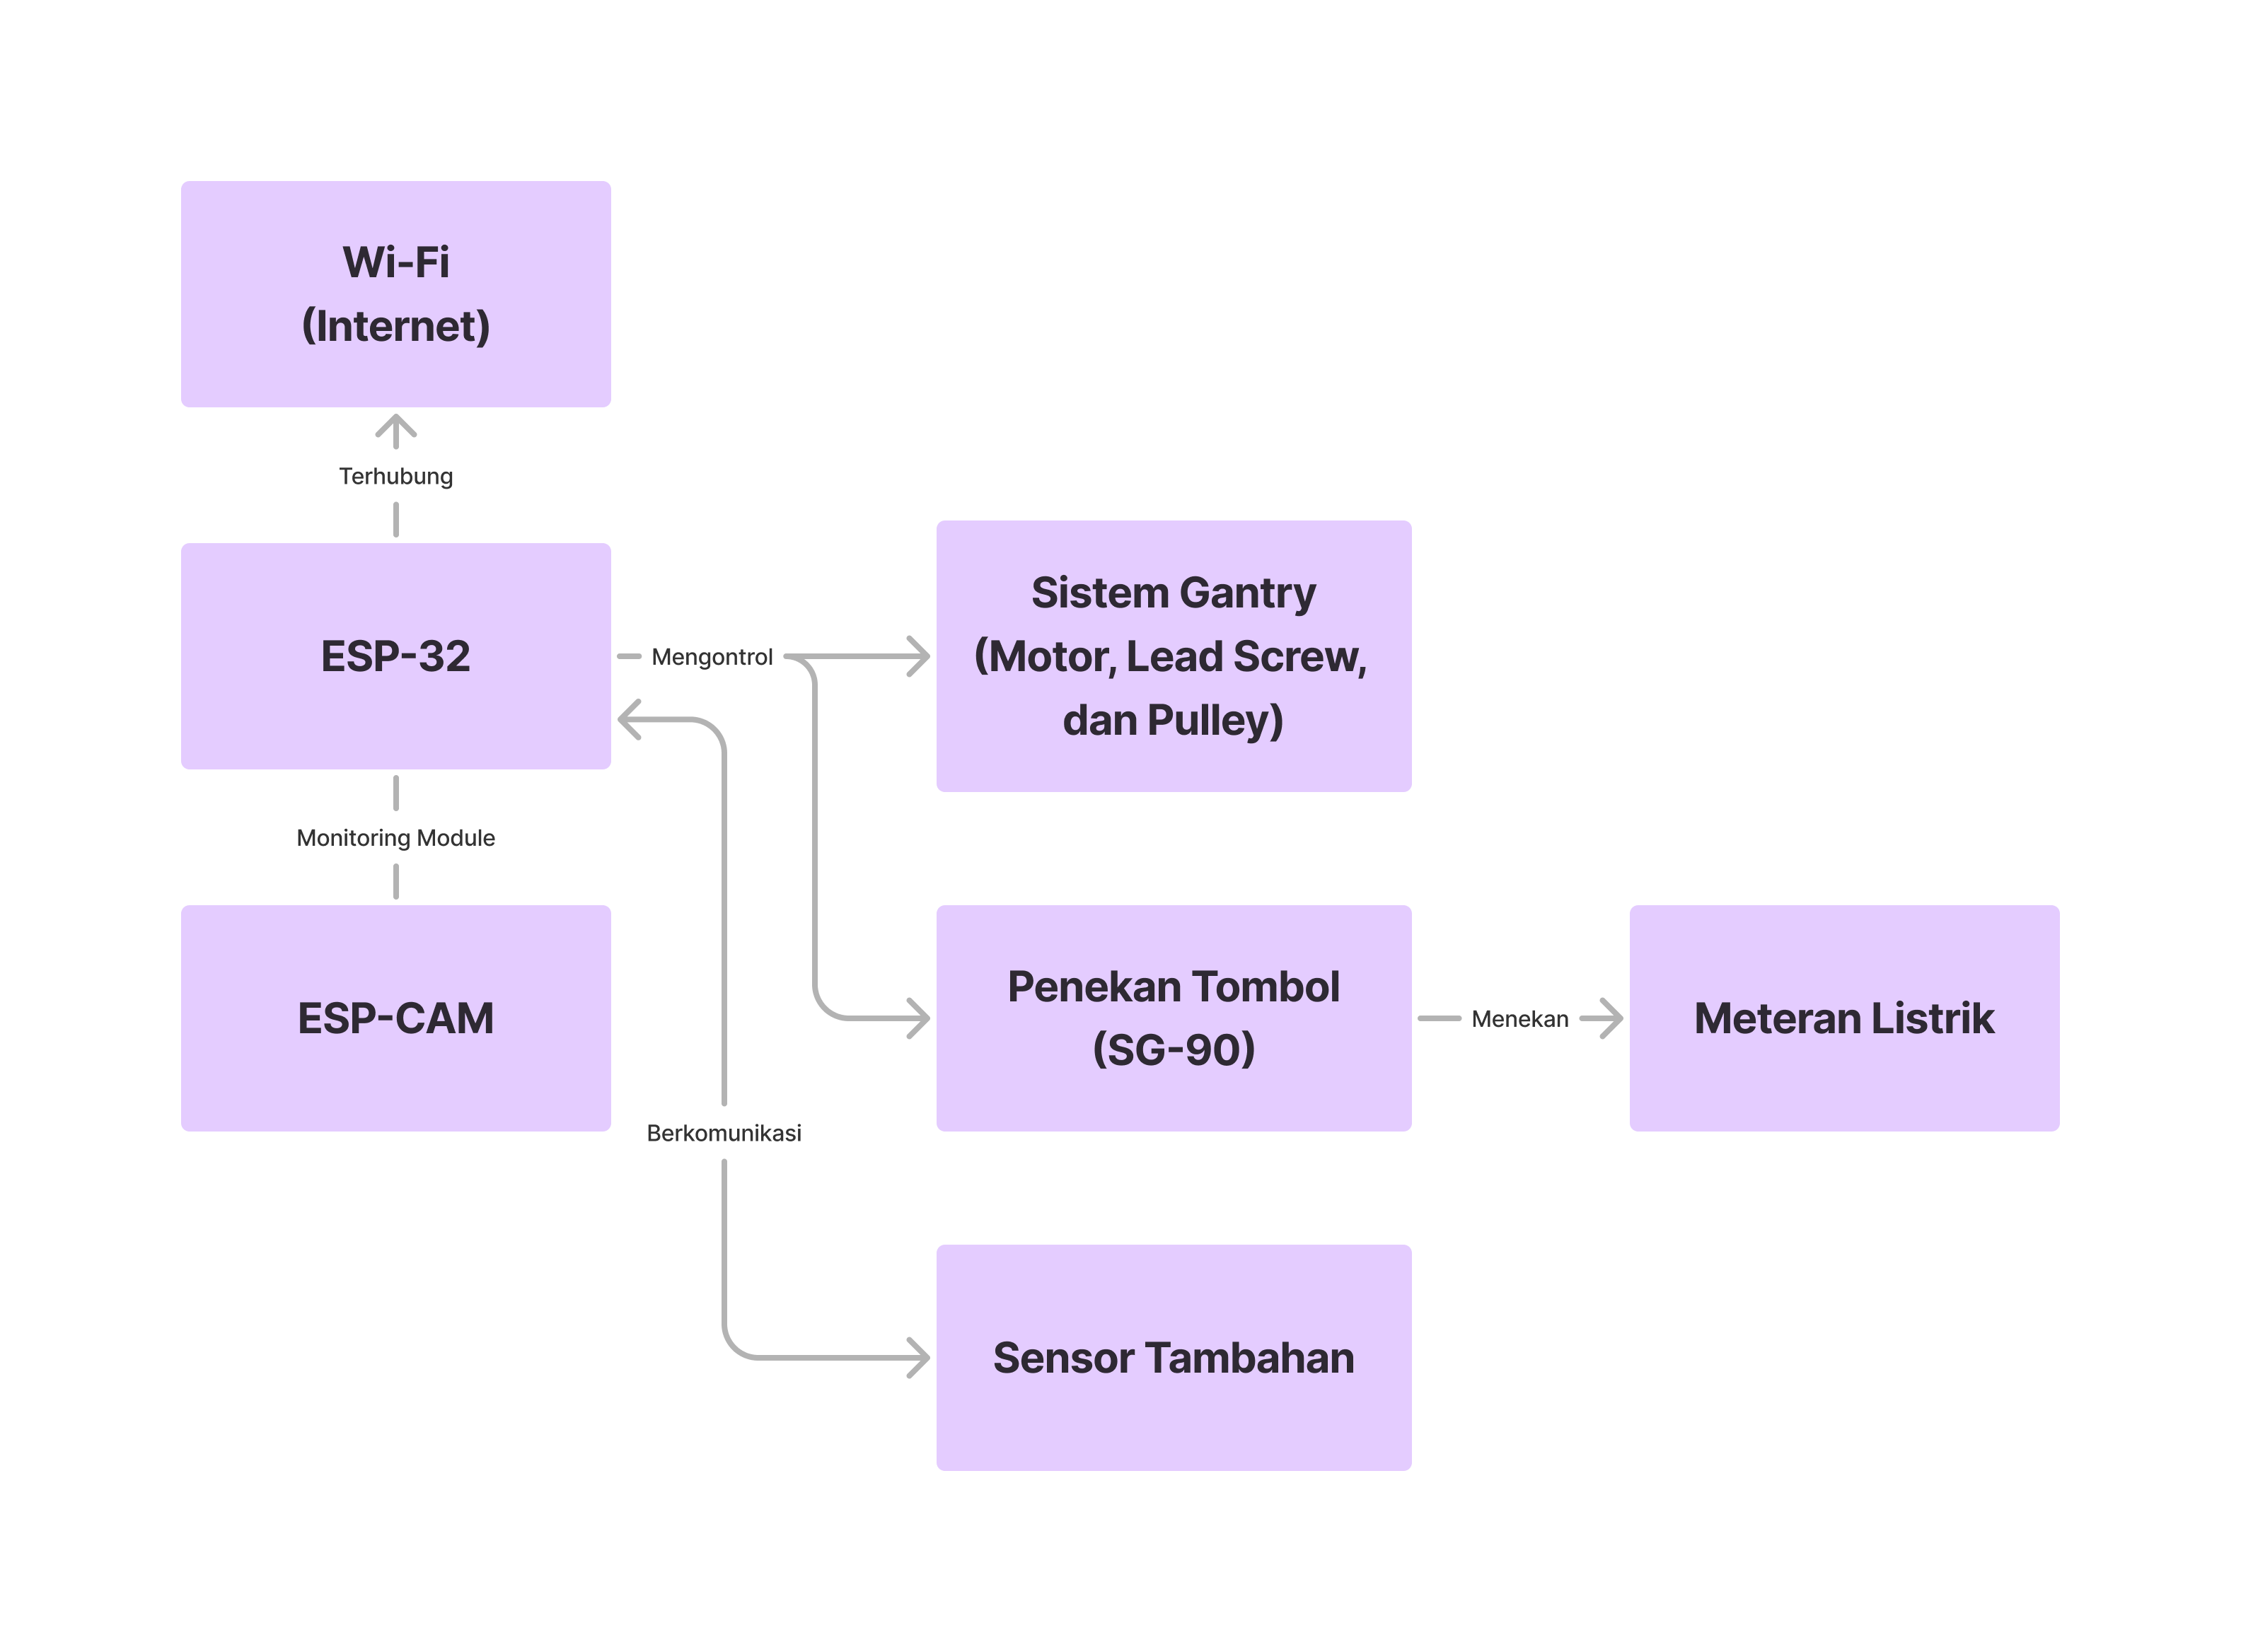
\includegraphics[width=1\linewidth]{gambar/implementasi-elektronik.png}
  \caption{Diagram hubungan komponen elektronik}
  \label{fig:implementasi-elektronik}
\end{figure}

Ada beberapa komponen elektronik yang digunakan dalam penelitian ini sesuai pada gambar \ref{fig:implementasi-elektronik},
beberapa diantaranya adalah
mikrokontoler \textit{ESP32} akan diprogram untuk menjalankan seluruh pergerakan dari alat, baik dari
pergerakan vertikal, horizontal, maupun penekanan tombol dari meteran listrik. \textit{ESP32} juga akan
terhubung ke internet melalui Wi-Fi sehingga pengguna dapat mengontrol alat dari jarak jauh. 
Kemudian motor yang digunakan
adalah motor \textit{stepper} NEMA-14 untuk pergerakan horizontal dan vertikal yang dikontrol menggunakan
\textit{motor driver} DRV8825, motor ini digunakan karena
ukurannya yang kecil dan cukup kuat untuk menggerakkan alat, salah satu motor tersebut akan dihubungkan
ke \textit{lead-screw} dan sekrupnya yang juga dibantu dengan \textit{guide rail} MGN12, 
yang menjadi penggerak vertikal utama dari alat, dan motor lainnya
akan terhubung ke sistem \textit{pulley} yang menjadi penggerak horizontal dari alat. kemudian motor 
\textit{servo} SG-90 untuk penekanan tombol pada meteran listrik, motor ini digunakan karena ukurannya 
yang kecil dan cukup kuat dengan \textit{torque} 1.98 kg/cm. 
Kemudian akan digunakan juga ESP-CAM sebagai sarana monitoring jarak jauh
dari alat, ESP-CAM ini digunakan karena kemampuannya yang dapat mengirimkan 
data melalui jaringan \textit{Wi-Fi}.
Penulis juga berencana untuk menggunakan beberapa sensor tambahan, seperti sensor jarak ultrasonik,
yang difungsikan sebagai sarana kalibrasi dan pengukuran jarak dari alat ke meteran listrik,
memastikan penggunaan alat dapat akurat dan presisi. Namun, sensor ini masih dalam tahap pengujian
sehingga belum diimplementasikan dalam prototipe. Kemudian baterai lithium-ion akan digunakan sebagai
sumber daya dari alat, sehingga alat dapat dipasang secara portabel tanpa perlu terhubung ke sumber listrik AC.

\section{Pemrograman Alat}

\begin{figure}[H]
  \centering
  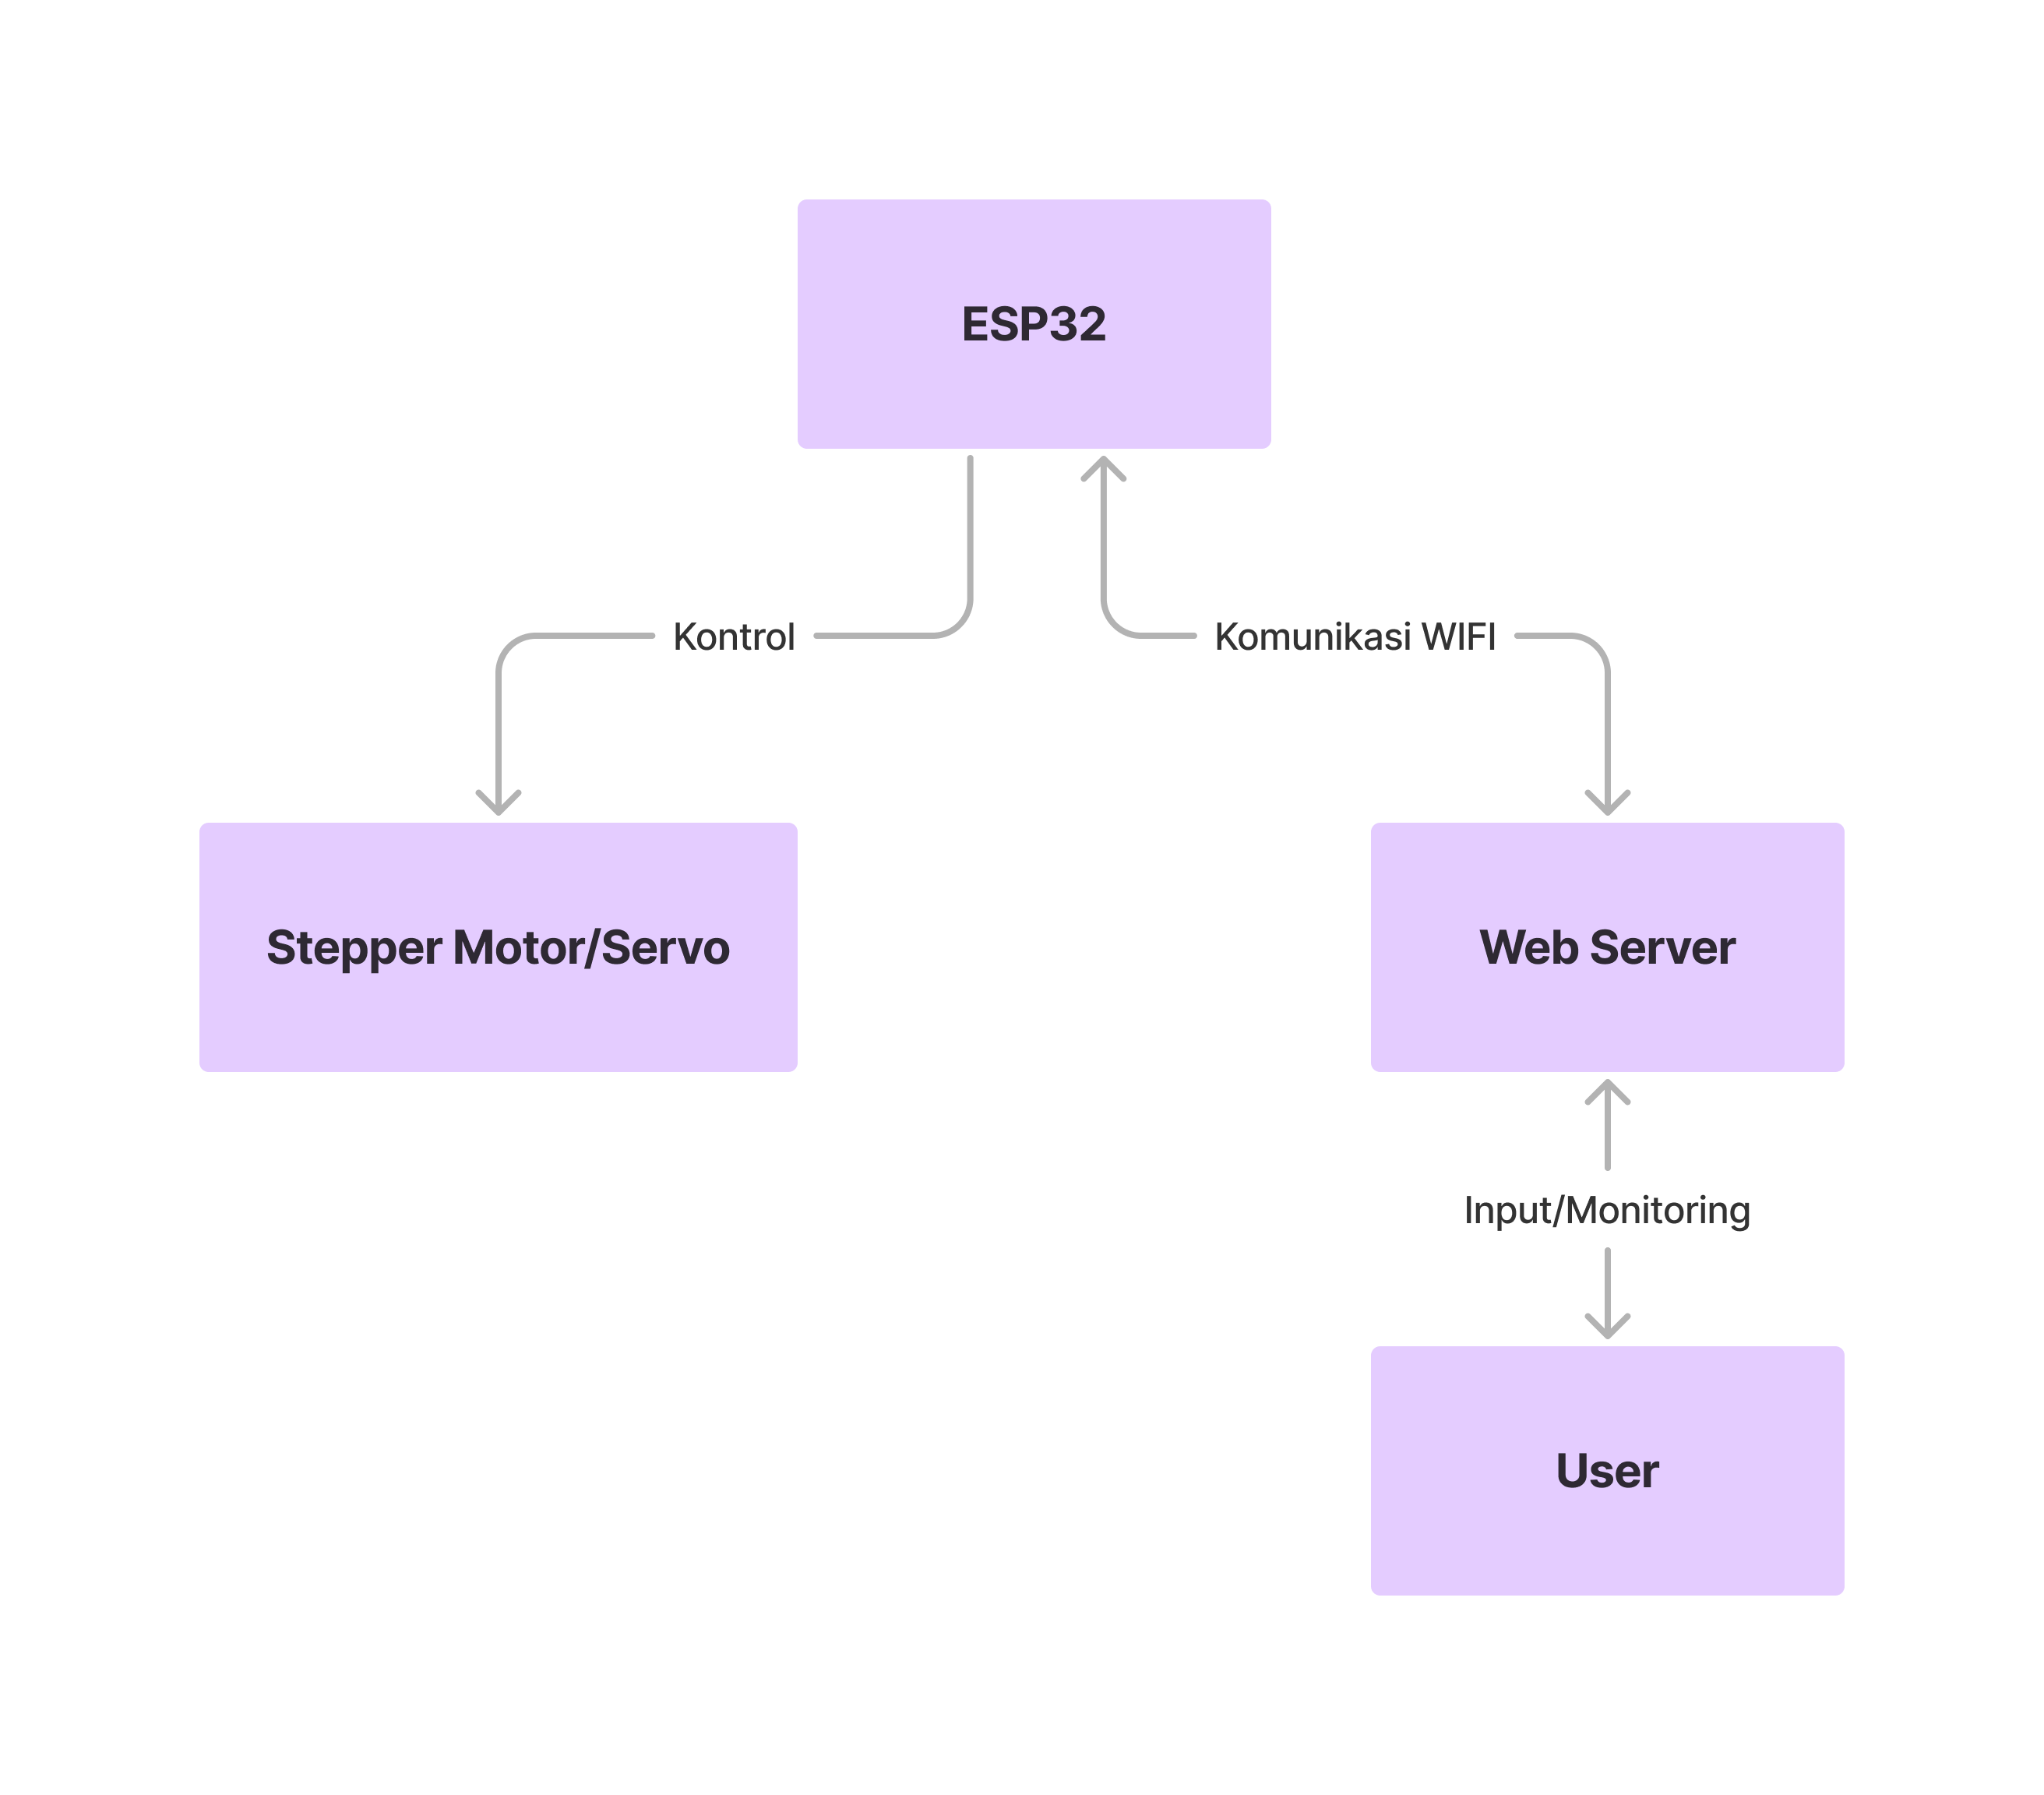
\includegraphics[width=0.8\linewidth]{gambar/diagram-program.png}
  \caption{Diagram hubungan program alat}
  \label{fig:diagram-program}
\end{figure}

Pemrograman alat dilakukan dengan menggunakan \textit{Arduino IDE} langsung menuju ESP32, kemudian komponen listrik
seperti motor stepper dan servo akan diatur menggunakan \textit{library} yang sudah disediakan oleh \textit{Arduino IDE}.
Beberapa dari \textit{library} yang digunakan adalah \textit{AccelStepper.h} untuk motor stepper (yang terhubung ke driver motor), 
\textit{Servo.h} untuk motor servo, dan \textit{WiFi.h} untuk koneksi internet. 

Secara garis besar,
algoritma yang digunakan diawali dengan memastikan koneksi internet terhubung, kemudian dilakukan
kalibrasi dari motor stepper dan servo memastikan jarak maksimum dari masing masing motor dan posisi
angka dari meteran listrik, untuk kalibrasi pergerakan vertikal dan horizontal dapat digunakan tombol yang menentukan titik
maksimum dan minimum dari posisi alat, sedangkan kalibrasi posisi tombol dapat dilakukan dari \texit{web interface} secara manual,
memastikan alat dapat digunakan di berbagai meteran listrik prabayar.
kemudian pengguna memberikan input melalui \textit{web interface}/aplikasi yang terhubung ke ESP32,
dan ESP32 akan menggerakkan motor stepper dan servo sesuai dengan input yang diberikan.

\section{\textit{Testing} dan Perbaikan}

Test
  \cleardoublepage

  % Konten lainnya
  \chapter{HASIL YANG DIHARAPKAN}

\section{Hasil yang Diharapkan dari Penelitian}

Dari penelitian yang akan dilakukan, diharapkan \lipsum[15]

\section{Hasil Pendahuluan}

Sampai saat ini, kami telah \lipsum[16]

  \cleardoublepage

  \chapter{JADWAL PENELITIAN}

% Ubah tabel berikut sesuai dengan isi dari rencana kerja
\newcommand{\w}{}
\newcommand{\G}{\cellcolor{gray}}
\begin{table}[H]
  \captionof{table}{Tabel timeline}
  \label{tbl:timeline}
  \begin{tabular}{|p{3.5cm}|c|c|c|c|c|c|c|c|c|c|c|c|c|c|c|c|}

    \hline
    \multirow{2}{*}{Kegiatan} & \multicolumn{16}{|c|}{Minggu}                                                                       \\
    \cline{2-17}              &
    1                         & 2                             & 3  & 4  & 5  & 6  & 7  & 8  & 9  & 10 & 11 & 12 & 13 & 14 & 15 & 16 \\
    \hline

    % Gunakan \G untuk mengisi sel dan \w untuk mengosongkan sel
    Pengambilan data          &
    \G                        & \G                            & \G & \G & \w & \w & \w & \w & \w & \w & \w & \w & \w & \w & \w & \w \\
    \hline

    Pengolahan data           &
    \w                        & \w                            & \w & \w & \G & \G & \G & \G & \w & \w & \w & \w & \w & \w & \w & \w \\
    \hline

    Analisa data              &
    \w                        & \w                            & \w & \w & \w & \w & \w & \w & \G & \G & \G & \G & \w & \w & \w & \w \\
    \hline

    Evaluasi penelitian       &
    \w                        & \w                            & \w & \w & \w & \w & \w & \w & \w & \w & \w & \w & \G & \G & \G & \G \\
    \hline
  \end{tabular}
\end{table}

Pada \emph{timeline} yang tertera di Tabel \ref{tbl:timeline} \lipsum[10]

  \cleardoublepage

  % Daftar pustaka
  \chapter*{DAFTAR PUSTAKA}
  \addcontentsline{toc}{chapter}{DAFTAR PUSTAKA}
  \renewcommand\refname{}
  \vspace{2ex}
  \renewcommand{\bibname}{}
  \begingroup
    \def\chapter*#1{}
    \printbibliography
  \endgroup


\end{document}
